\documentclass{book}

%%%%%%%%%%%%%%%%%%%% Packages %%%%%%%%%%%%%%%%%%%%

\usepackage[utf8]{inputenc}
\usepackage[T1]{fontenc}
\usepackage[french]{babel}
\usepackage{graphicx}
\usepackage{geometry}
\usepackage{enumitem}
\usepackage{xcolor}
\usepackage{pdfpages}
\usepackage{tikz}
\usepackage{stmaryrd}
\usepackage{amsmath}
\usepackage{lmodern}
\usepackage{amssymb}
\usepackage{mathrsfs}
\usepackage{colortbl}
\usepackage{mathabx}
%\usepackage{txfonts}

\usepackage{booktabs}
\usepackage{longtable}
\usepackage{array}
\usepackage{multirow}
\usepackage{wrapfig}
\usepackage{float}
\usepackage{colortbl}
\usepackage{pdflscape}
\usepackage{tabu}
\usepackage{threeparttable}
\usepackage{threeparttablex}
\usepackage[normalem]{ulem}
\usepackage{makecell}

%%%%%%%%%%%%%%%%%%%%%%%%%%%%%%%%%%%%%
%%%%%%%%%% Pour biblio %%%%%%%%%%%%%%
%%%%%%%%%%%%%%%%%%%%%%%%%%%%%%%%%%%%%




%%%% Pour toc %%%%
\addtocounter{tocdepth}{3}
\setcounter{secnumdepth}{3}
\addcontentsline{toc}{section}{Introduction}
\addcontentsline{toc}{section}{Remerciements}
\addcontentsline{toc}{section}{Citations}
\renewcommand{\thesection}{\arabic{section}}




%%%%%%%%%%%%%%%%%%%% Page de Garde %%%%%%%%%%%%%%%%%%%%    
\author{\textbf{Odélia Guedj} \\ M1 Mathématiques en Interaction \\ Université Evry Val d'Essonne}
\title{\LARGE{Étude de l'impact de l'activité professionnelle sur la santé perçue dans la cohorte EPP3}}
\date{01/04/2019 - 31/08/2019}

\makeatletter
\let\mytitle\@title
\let\myauthor\@author
\let\mydate\@date
\makeatother

\begin{document}
\begin{titlepage}

\enlargethispage{10 cm}


\includegraphics[scale = .4]{logo_inserm.jpg}\hfill

\includegraphics[scale = .2]{logo_parcc.jpg}\hfill

\includegraphics[scale = .4]{logo_ueve_saclay.png}
\\ \\ \\ \\ \\ \\ \\ \\ \\ \\

\begin{center}
\begin{tabular}{c}
\hline
\hline
\LARGE{Étude de l'impact de l'activité professionnelle sur la santé perçue} \\
\\
\LARGE{des sujets de la cohorte EPP3}. \\
\hline
\hline
\end{tabular}
\end{center}

\begin{minipage}\linewidth
        \centering\sffamily
        \normalsize{INSERM U970 PARCC (Paris Centre Cardiovascualaire)}
        \vskip3pt 
        E04 : Integrative Epidemiology of Cardiovascular Deseases\\
    \end{minipage}
    
\begin{center}
\normalsize{\textbf{\mydate}}\\
\end{center}

\bigskip
\begin{center}
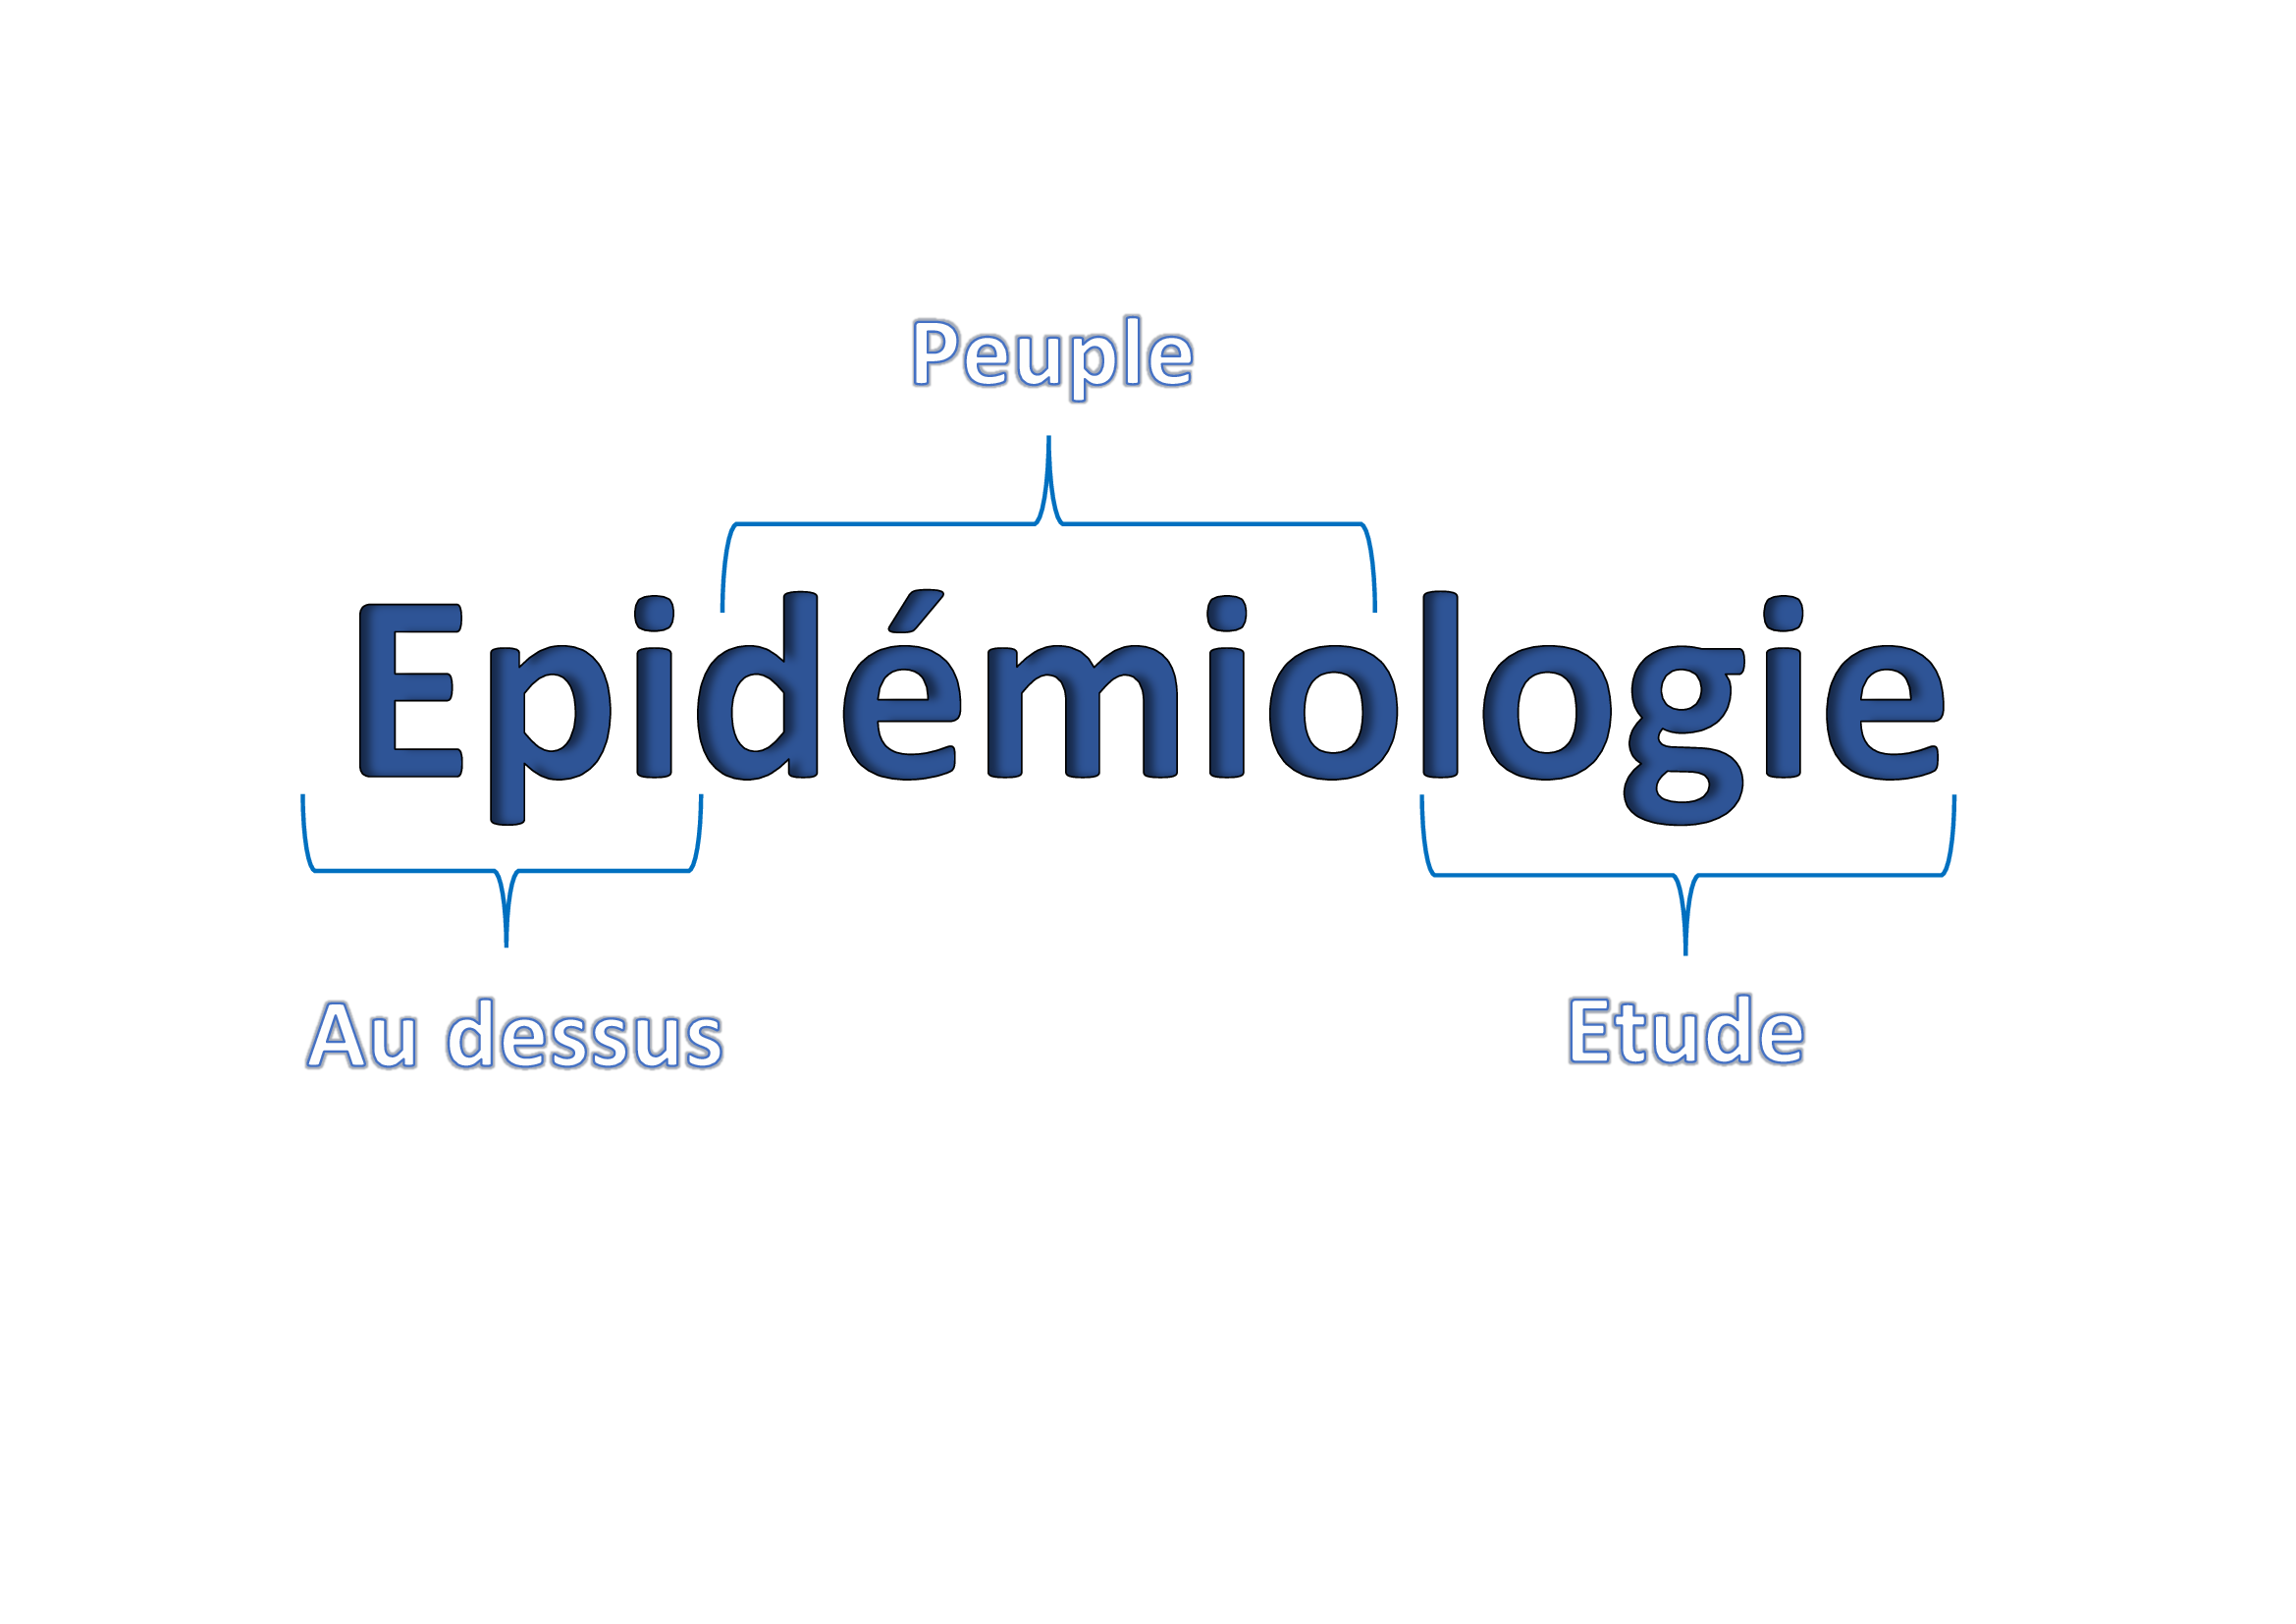
\includegraphics[scale= .1]{Epidemiologie_logo_im.png}
\end{center}


\begin{tabular}{p{.5\textwidth}p{.5\textwidth}}
\flushleft \myauthor \\ 
& \flushright \textbf{Dr Jean Philippe Empana} \\ Research Director, MD, PhD \\ INSERM U970 PARCC
\end{tabular}


\end{titlepage}
 
%%%%%%%%%%%%%%%%%% frontmatter %%%%%%%%%%%%%%%%%%%
\frontmatter

\tableofcontents

\newpage
\begin{center}
\section*{Remerciements}
\end{center}
\bigskip

\noindent
Je tiens à remercier l'ensemble des personnes ayant contribué au sucés de ce stage.\\

\noindent
Tous d'abord, merci au Dr Jean Philippe Empana de m'avoir fait confiance en m'accueillant dans son équipe. 
J'y ai énormément appris tant sur le plan statistique que sur le plan humain. J'ai découvert avec beaucoup de plaisir le monde de la recherche où j'espère un jour me faire une place !
Merci d'avoir toujours pris le temps de répondre à mes questions et surtout de m'avoir laissé assez de liberté pour que je découvre des choses par moi même.\\

\noindent
Je tiens également à remercier Marie Lê Hoang, Ingénieur d'étude à l'INSERM qui a gentiment accepté de faire circuler mon CV dans l'unité et grâce à qui j'ai eu la chance d'avoir 3 propositions de stages.\\

\noindent
Un grand merci à toute l'équipe 4 de l'unité pour ces 5 mois passés ensemble: des heures de discussions méthodologie, statistiques, éthique et médecine. Des heures à dompter des bouts de codes capricieux qui ne font pas ce qu'on leur demande. Merci pour cette ambiance de travail dans la bonne humeur : Bamba Gaye (MD, Phd), Marie-Aude Penet (MD, MSc), Prunelle Getten (MD, MSc), Willy Sutter (MD, PhD), Delphine Lavignasse (PhD), Anouk Asselin (MSc), Marie-Cécile Perrier(MSc), Lucile Ofredo (MSc), Radia B(ARC) ainsi que tous les apprentis chercheurs de passage.\\

\noindent
Enfin, merci à Mme Agathe Guilloux et Mme Marie Luce TAUPIN, Enseignants Chercheurs à l'Université d'Évry Val 
d'Essonne pour leur aide durant cette année un peu particulière. Merci pour votre compréhension et pour le temps que vous m'avez accordé.


\newpage
\begin{center}
\section*{Citations}
\end{center} 

\bigskip


\begin{flushright}
\textit{Nous ne devons pas laisser croire que tout progrès scientifique peut être réduit à des mécanismes, des machines, des rouages, quand bien même de tels mécanismes ont eux aussi leur beauté.}
\textbf{Madame Curie, Ève Curie, éd. Gallimard, 1938}
\end{flushright}

\bigskip
\begin{flushright}
\textit{The new form of the problem can be described in terms of a game which we call the 'imitation game."\\
It is played with three people, a man (A), a woman (B), and an interrogator (C) who may be of either sex.\\
The interrogator stays in a room apart front the other two. The object of the game for the interrogator is to determine which of the other two is the man and which is the woman. He knows them by labels X and Y, and at the end of the game he says either "X is A and Y is B" or "X is B and Y is A."\\
The interrogator is allowed to put questions to A and B...\\
We now ask the question, "What will happen when a machine takes the part of A in this game?"\\
Will the interrogator decide wrongly as often when the game is played like this as he does when the game is played between a man and a woman?\\
These questions replace our original, "Can machines think?"}\\
\textbf{Mechanical Intelligence: Collected Works of A.M. Turing}
\end{flushright}


%%%%%%%%%%%%%%%%%%%% main matter %%%%%%%%%%%%%%%%%%%%%%%%%%%%%%%%
\mainmatter


\newpage
\begin{center}
\section*{Introduction}
\end{center}

\noindent
Les retraités : leur nombre, leur âge, le montant de leur pension sont des sujets récurrents des derniers mandats présidentiels français.\\
Les récentes législations\cite{noauthor_code_nodate} concernant le recul de l'âge légal du départ à la retraite se sont vues opposer de violentes résistances qui posent la question de la santé des individus actifs par rapport à celle des retraités\cite{fatas_experimental_2007} .\\

\noindent
La santé perçue, Self Rated Health en anglais, est une mesure subjective de la santé des individus souvent utilisée en santé publique.\\
Cette mesure est effectuée grâce à une question directe aux individus : Sur une échelle de 0 à 10, comment évaluez vous votre santé (avec 0: très mauvaise et 10 excellente).\\
La santé perçue est décrite dans la littérature comme un indicateur consistant de mortalité\cite{mossey_self-rated_1982} \cite{crossley_reliability_2002} ayant des liens fort avec la santé mentale \cite{millan-calenti_depressive_2012} et le contexte socio-économique des individus \cite{mansyur_social_2008} \cite{alvarez-galvez_impact_2013}.\\
Si la santé perçue reflète assez bien la santé objective d'individus \cite{wu_relationship_2013} , il est important de souligner que sa nature subjective en fait un outils plus puissant encore puisqu'il permet de prendre en compte des critères psychologiques et sociaux comme les habitudes alimentaires, l'historique familial ou les disposition à la sur/sous évaluation d'un risque.\\

\noindent
Cet outils a été utilisé dans l'étude de la cohorte GAZEL pour mettre en évidence l'hypothèse suivante\cite{westerlund_self-rated_2009}  : les individus actifs voient leur santé perçue augmenter après avoir pris leur retraite. Pour ce faire les investigateurs disposaient de plusieurs points de mesure avant et après la retraite des sujets de la cohorte GAZEL.\\

\noindent
L'objectif de mon stage était de m'inspirer des hypothèse de l'étude décrite ci-dessus pour montrer que la santé perçue des individus de l'Etude Parisienne Prospective 3 \cite{empana_paris_2011} est impactée par leur activité professionnelle.\\



\newpage
\section{Contexte}
\subsection{L'Inserm U970 Équipe 4}

\noindent
L'INSERM : Institut National de la Santé Et de la Recherche Médicale est un établissement publique de recherche créé en 1964 par le ministre de la santé Raymond Marcellin et dont la santé Publique et l'épidémiologie sont un des domaines de spécialité.\\
L'INSERM est constitué de plusieurs dizaines d'unités réparties sur l'ensemble du territoire français et dont le siège se trouve rue Tolbiac dans le 13 ème arrondissement de Paris.\\
J'ai effectué mon stage au PARCC (Paris Centre Cardiovasculaire): une unité mixte de recherche de l'INSERM (U970) située dans le bâtiment recherche de l'hôpital George Pompidou (Rue Leblanc Paris 15) depuis 2009.\\
Cette unité est composée d'une dizaine d'équipes ayant une "vocation\footnote{Site Web de l'Hôpital Européen George Pompidou} internationale dans le domaine de la recherche fondamentale et translationnelle sur les maladies cardiovasculaires, à partir d'approches multiples combinant biochimie, biologie cellulaire et moléculaire, imagerie moléculaire, physiologie intégrative, pharmacologie, génétique et épidémiologie".\\

\noindent
Durant mon stage j'ai intégré l'équipe 4: Integrative Epidemiology of Cardiovascular Deseases, co-dirigée par le Dr Jean Philippe Empana et le Dr Xavier Jouven dont les sujets de recherche peuvent être résumés en quatre points:
\noindent
\begin{enumerate}
\item CEMS : Centre d'Expertise de la Mort Subite. Il s'agit de la création d'une base de données recensant de façon exhaustive les événements de mort subite de Paris et de la petite couronne.\\
\item Approche multi-marqueurs à la détection de nouveaux facteurs de risque aux maladies cardiovasculaires.\\
\item Épidémiologie des maladies cardiovasculaires dans les pays en voie de développement.\\
\item The Paris Transplant Group : Epidémiologie de l'immuno-atherosclerosis.\\
\end{enumerate}

Ma recherche est inclue dans le deuxième point ci dessus.\\

\noindent
L'équipe est composée de médecins, de statisticiens, d'attachés de recherche clinique (ARC) et d'étudiants (thèse de science, stage M1/M2, post-doc).\\
On y trouve une grande diversité de nationalités, de parcours, de spécialités donnant une vue d'ensemble sur le monde de la recherche en santé/bio-statistiques et créant une émulsion qui m'a beaucoup profité.\\

%\noindent
%La pluralités des parcours des personnes composant l'équipe participe largement au plaisir que j'ai eu à y %travaille. J'ai pu profiter de l'émulsion qu'un tel environnement de travail occasionne.\\
%\noindent
%Pouvoir partager ses idées, les confronter à d'autres points de vues et surtout se soucier de la pertinence clinique de certaines analyses a été un véritable enrichissement. En effet, les médecins de l'équipe se sont montré très ouverts à la vulgarisation de certaines notions médicales de base qui m'ont permis et me permettront de mieux appréhender le sens de mes données. Dans la même dynamique, les statisticiens (en l'occurrence statisticiennes) de l'équipe m'ont fait découvrir nombre de méthodes et d'astuces qui ont sensiblement enrichi mes compétences.\\

%De plus, chaque semaine, des séminaires scientifiques sur les maladies cardiovasculaires sont organisés. La %plupart du temps il s'agit de biologie fondamentale. Cependant j'ai parfois eu l'occasion d'écouter des %intervenants moins "théoriques" par exemple sur l'état actuel de la recherche dans le domaine cardio %vasculaire. Ces contact avec des chercheurs et l'exposition de leurs travaux m'a été très bénéfique ne serait-%ce que pour comprendre comment fonctionne le monde de la recherche en France et à l'international.\\

%J'ai également eu la possibilité de participer à des réunions de méthodologie desquelles j'ai énormément %appris. L'exercice consistait à une lecture critique d'article. Chacun des participants lit l'article puis lors %d'une réunion en expose ce qu'il a compris et surtout ce qui lui semble flou. On se concentre particulièrement %sur la partie méthodologie de l'article qui expose les outils statistiques utilisés par les auteurs pour mener %à bien leur analyse : comment ils ont recueillis les données, comment ils o,t co,struot leur variables, quel %model est  tilisé... En essayant de lire les tables de résultats, certaines critiques apparaissent

%Beaucoup d'émulsion: ouverture sur méthodes stats, vulgarisation notions de médecine. Équipe humaine, agréable.\\
\subsection{L'étude Parisienne Prospective 3 (EPP3)}
\noindent
EPP3 \cite{empana_paris_2011} est une étude prospective de cohorte en population générale comptant n = 10157 sujets.\\
Ces dernier ont été recrutés dans des centres IPC (centres d'examens de santé conventionnés par l'assurance maladie) entre Juin 2008 et Décembre 2011.\\
Pour entrer dans l'étude, les sujets doivent avoir entre 50 et 75 ans.\\
\\
Les données sont récoltées via des questionnaires envoyés tous les deux ans qui, à l'exception du questionnaire d'inclusion sont élaborés à l'INSERM U970 équipe 4. \\
Le questionnaire d'inclusion\footnote{Annexe 1} provient de l'IPC. Il contient une partie socio-admnistrative, des questions sur l'environnement professionnel des sujets ainsi que sur leurs habitudes de vie (alimentation, tabac, alcool). 
Une autre partie du questionnaire traite des antécédents médicaux des sujets, tant familiaux que personnels, de leur état de santé actuel et de leurs prescriptions médicamenteuses.
La dernière partie traite du bien-être des sujets: on y trouve des questions sur leur stress perçu, leur équilibre mental ainsi que leur nutrition.\\
\\
Le but de l'étude est la recherche de facteurs de risque pour les maladies cardiovasculaires.\\ 
Dans chacun des questionnaires il est demandé aux sujets de déclarer leurs hospitalisations en détaillant le motif d'hospitalisation, le nom de l'hôpital, du service où ils ont été traités ...\\
Chaque hospitalisation déclarée est appelée évènement.\\
\\
Pour s'assurer de la validité des déclarations des sujets, un protocole de validation d'événement a été mis en place : régulièrement un certain nombre d'événements sont extraits de la base. Pour chaque évènement, on contacte l'hôpital pour qu'il transmette au responsable de l'étude les comptes-rendus hospitaliers (CRH) de l'évènement en question. Ensuite les CRH sont lus par un médecin qui valide, invalide ou corrige le diagnostique déclaré par le sujet.\\
\\
L'étude EPP3 est une étude longue, il est prévu que le suivi dure 20 ans (10 questionnaires à raison d'un tous les deux ans).\\
Elle a déjà donné lieu à la publication de plus d'une vingtaine d'articles dans des revues prestigieuses comme le JACC (Journal of the American College of Cardiology) ou le JAMA (Journal of the American Medical Association).\\

\newpage
\section{Bref aperçu de l'épidémiologie}

\subsection{Histoire et définition}

\noindent
Épidémiologie vient des mots grecs "epi": au-dessus, "demio": peuple. Ainsi la définition étymologique de l'épidémiologie est l'étude des peuples.\\
Si l'on tente de donner une définition plus précise de ce qu'est l'épidémiologie on se retrouve vite enseveli sous le nombre de possibilités.\\

\noindent
Le dictionnaire Larousse propose la définition suivante: \textit{Science qui étudie, au sens des populations (humaines, animales voir végétales), la fréquence et la répartition des problèmes de santé dans le temps et dans l'espace, ainsi que le rôle des facteurs qui les déterminent}.\\

\noindent
Cependant deux autres définition méritent d'être citées pour leur pertinence (préférence subjective bien entendu). Celle Mac Mahon : \textit{Étude de la distribution et des déterminants d'une maladie dans des populations humaines, et application des résultats de cette étude dans la lutte contre cette maladie}, et celle de Jeniceck : \textit{L'épidémiologie est un raisonnement et une méthode propres au travail objectif en médecine et dans d'autres sciences de la santé, appliqués à la description des phénomènes de santé, à l'explication de leur étiologie, et à la recherche des méthodes d'intervention les plus efficaces}.\\

\noindent
Ce cocasse problème de définition est cependant assez sérieux pour que des épidémiologistes décident de mener leur enquête \cite{frerot_what_2018} sur les définitions données à leur discipline entre 1978 et 2017. Ils en répertorient 102 et identifient 5 termes présent dans plus de la moitié des définitions répertoriées: "population", "étude", "santé","maladie" et "distribution".\\
Ils observent également une augmentation des mots "contrôle" et "santé" dans les définitions entre 1978 et 2017. Il est à noter que les définitions autorisées à être inclues dans l'étude sont soit en anglais soient des définitions nationales traduites en anglais.\\

\noindent
Les 5 mots cités précédemment rendent assez bien compte de ce qu'est réellement la discipline, preuve que l'étude menée sur ses définitions n'était pas vaine puisqu'elle permet de comprendre en profondeur ce qu'est l'épidémiologie (santé, maladie, étude), en quoi elle se détache de la médecine (population, distribution) et pourquoi elle est utile (contrôle,maladie).\\

\noindent
Forts de ces éclaircissements, nous pouvons sans trop nous tromper, faire l'hypothèse que l'épidémiologie est aussi vieille que la médecine. Depuis la discipline a beaucoup évolué, s'adaptant aux nouveaux défis posés par l'apparition de maladies.\\

\noindent
Dans un article de médecine science publié en 2016  \cite{bizouarn_leco-epidemiologie_2016}, Philippe Bizouarn\footnote{Épidémiologiste, Praticien hospitalier - Service d’Anesthésie-Réanimation de l’Hôpital G et R Laënnec, CHU de Nantes} identifie 4 aires distinctes de l'épidémiologie.\\
La première appelée statistiques sanitaires repose sur la théorie des miasmes (émanations fétides du sol, de l'air, de l'eau) et occupe la deuxième moitié du XIX$^{ème}$ siècle.\\

\noindent
La seconde, ère des maladies infectieuses, s'étend de la deuxième moitié du XIX$^{ème}$ siècle à la deuxième moitié du XX$^{ème}$ siècle. Elle rejette la théorie des miasmes au profit de la théorie des germes avec la découverte du microbe.\\
Un exemple historique d'étude épidémiologique de cette ère est celle que J.Snow effectue en 1954 afin de mettre en évidence le mode de propagation du choléra. Il découvre un lien fort entre le nombre de cas de choléra dans une zone et la distribution d'eau qui la dessert. Il arrive à prouver qu'une des pompes d'eau occasionne le plus grand nombre de cas de choléra, la fait retirer et endigue ainsi l'épidémie. L'eau est alors communément admise comme voie de propagation de la maladie.\\

\noindent
La troisième ère de l'épidémiologie identifiée par P.Bizouarn (deuxième moitié du XX$^{ème}$ siècle jusqu'au début du XXI$^{ème}$) est celle des maladies chroniques dont une des études les plus connues est celle de Dull et Hill datant de 1950 sur le cancer bronchopulmonaire.\\

\noindent
Enfin il appelle la dernière ère, l'ère de l'éco-épidémiologie caractérisée par la recherche et l'analyse des associations entre plusieurs "facteurs de risques" (par exemple l'exposition à une maladie, le tabac, l'alcool...) et les "issues" (maladies) sans rechercher systématiquement de "lien causal" entre un des facteurs et les issues.\\


\subsection{Notions de base, vocabulaire}

\noindent
L'épidémiologie utilise des méthodes statistiques afin de décrire une maladie ou d'en rechercher les causes. Cependant, le vocabulaire utilisé diffère quelque peu de celui utilisé en mathématiques.\\
Ainsi la variable à expliquer, $Y$, est souvent appelée variable d'intérêt. \\

\noindent
De plus, en épidémiologie, les variables explicatives, ou covariables, sont classées dans plusieurs groupes:

\begin{itemize}
\item Il y a d'une part la variable d'exposition c'est à dire la variable explicative principale. 
\item Les facteurs de confusion: ce sont les covariables qui sont inclues de façon (quasi) systématiques dans les modèles statistiques pour des raisons cliniques. Ces variables sont décrites dans la littérature et varient selon la branche médicale. On y retrouve souvent l'âge, le sexe, l'indice de masse corporelle des sujets ainsi que leur habitudes de vie: tabac, alcool, score de dépression, statut marital...\\
Les facteurs de confusion sont des variables à la fois liées au facteur de risque et à la variable d'intérêt.
\item Enfin les autres variables explicatives sont appelées variables d'ajustement: il s'agit d'autres facteurs pouvant participer, avec la variable d'exposition, à l'explication de la variable d'intérêt.
\end{itemize} 

\bigskip 

\noindent
L'épidémiologie a deux champs principaux d'application:
\begin{itemize}
\item \textit{L'épidémiologie classique} qui décrit et mesure des phénomènes de santé dans une population. Elle a pour but l'élaboration de stratégies de santé publique.
\item \textit{L'épidémiologie clinique} dont les études se concentrent sur des populations de patients en vue d'améliorer les connaissances d'une maladie ou de tester l'efficacité d'un traitement.
\end{itemize}

\newpage

L'épidémiologie se décompose en trois branches:
\begin{enumerate}
\item \textit{L'épidémiologie descriptive} qui consiste en l'étude de la fréquence et de la répartition de phénomènes de santé.  Elle permet de formuler des hypothèses quant aux causes de ces phénomènes.
\item L'épidémiologie analytique dont le but est de vérifier les hypothèses susmentionnées. Elle recherche les liens entre l'exposition à un facteur et la survenue d'un phénomène de santé.
\item \textit{L'épidémiologie évaluative} qui mesure l'efficacité d'une intervention (thérapeutique ou de prévention) sur le phénomène de santé.
\end{enumerate}

\bigskip

Une étude épidémiologique peut se faire deux manières :
\begin{itemize}
\item En observant les effets sur une population de l'exposition de facteurs de risques : on parle d'\textit{observation}.
\item En contrôlant les conditions d'exposition à ces facteurs de risque : on parle d'\textit{étude expérimentale}.\\
\end{itemize}

\noindent
L'étude est dite \textit{randomisée} si le hasard seul est responsable de l'appartenance d'un sujet à un groupe. On parle d'une \textit{étude ouverte} quand le traitement est connu des sujets et des investigateurs, \textit{en simple aveugle} quand seuls les investigateurs connaissent le traitement et \textit{en double aveugle} lorsque ni les sujets ni les investigateurs ne connaissent le traitement.\\
Cependant les études expérimentales sont presque toujours irréalisables car non éthiques : une étude expérimentale sur le lien entre le tabac et l'apparition d'un cancer du poumon supposerait en effet d'exposer une partie de la population étudiée au tabac puis d'étudier les conséquences sur leur poumon.\\

\bigskip

Lorsque l'on fait de l'épidémiologie descriptive on peut faire deux sortes d'étude:
\begin{itemize}
\item Étudier la \textit{prévalence} d'un phénomène de santé, c'est à dire la fréquence de survenue de ce phénomène dans une certaine population à un temps donné. Dans ce type d'étude l'évolution temporelle n'existe pas, c'est une mesure effectuée à un temps donné: on parle d'\textit{étude transversale}.
\item Étudier l'\textit{incidence} d'un phénomène de santé, c'est à dire étudier les modifications de l'état de santé d'un ou de plusieurs groupes de sujets sur une période donnée. Ici c'est bien l'évolution dans le temps d'un état qui importe: on parle d'\textit{étude longitudinale}.
\end{itemize}

\bigskip

\noindent
Par ailleurs lorsque le but de l'étude épidémiologique est à visée étiologique on dénombre deux grandes familles d'étude:
\begin{itemize}
\item \textit{L'étude de cohorte}: Étude d'un groupe de personnes étant ou pouvant être exposé à un facteur de risque. C'est l'étude épidémiologique la plus exhaustive.
\item \textit{L'étude cas-témoin}: elle étudie la comparaison entre deux groupes : les malades appelés cas et les non-malades appelés témoins. Le but est de déterminer si la réponse à l'exposition à un facteur est similaire dans les deux sous-groupes et ainsi d'établir un lien facteur/maladie.
\end{itemize}

\bigskip

\noindent
Enfin, une étude peut être \textit{prospective} si  l'information concernant l'exposition des sujets à un facteur est recueillie avant la survenu d'un phénomène de  santé, ou \textit{rétrospective} si l'information concernant l'exposition des sujets à un facteur est recueillie après  la survenu d'un phénomène de  santé chez certains sujets.

\subsection{Principaux biais de l'épidémiologie}
\noindent
Un biais est une erreur de méthodologie commise le plus souvent durant l'inclusion des sujets dans l'étude et conduisant à une mauvaise estimation des paramètres étudiés.\\

\noindent
Il en existe 3 principaux:
\begin{itemize}
\item Le \textit{biais de sélection}: : Intervient lors de la constitution de l'échantillon d'enquête. C'est le biais induit par la manière dont les sujets sont choisis au sein de la population. 
\item Le \textit{biais de mesure}: due à une mauvaise mesure du facteur d'exposition.
\item Le \textit{biais de confusion}: due à la mauvaise analyse de la relation d'un facteur avec une issue. Un tel facteur est appelé facteur de confusion.
\end{itemize}

\section{Description et explication des données}
\noindent
Le but de cette analyse est d'établir l'existence d'un lien entre l'activité professionnelle des sujets d'EPP3 et la manière dont ils perçoivent leur santé. Si cette dernière fait l'objet d'une question claire dans le questionnaire d'inclusion, ce n'est pas le cas de l'activité professionnelle. J'ai ainsi dû créer une nouvelle variable en extrayant de l'information de plusieurs questions grâce à des méthodes de classifications non supervisées.\\
La description des méthodes utilisées à la mise en forme de l'ensemble des variables utiles à l'analyse fait l'objet de cette section.
\subsection{Variable d'exposition : Activité Professionnelle}
\noindent
Dans le questionnaire d'inclusion, 3 questions traitent de l'activité professionnelle des sujets (Question 1,2,3 du questionnaire IPC en annexe). Ces 3 questions ont été codées en 4 variables catégorielles :

\begin{small}
\begin{itemize}[label=\textbullet]
\item Adm12 : Êtes-vous
\begin{itemize}[label=\textbullet]
\item 6NNNNN  contrat emploi-solidarité, intérim, CDD
\item N5NNNN  chômeur depuis + de 6 mois
\item NN4NNN  chômeur depuis - de 6 mois
\item NNN3NN  à la recherche d'un emploi
\item NNNN2N  jeune en cours de formation
\item NNNNN1  étudiant
\end{itemize}

\bigskip

\item Adm12a : Êtes-vous
\begin{itemize}[label=\textbullet, font=\small]
\item JXXX  en formation professionnelle
\item X9XX  au foyer
\item XX8X  retraité(e)
\item XXX7  pré-retraité(e)
\end{itemize}

\bigskip

\item Adm11 : Depuis quand n'exercez-vous plus d'activité professionnelle ?
\begin{itemize}[label=\textbullet, font=\small]
\item 0	en activité
\item 1	moins d'un an
\item 2	1 an
\item 3	2 ans
\item 4	3 ans ou +
\item 5	jamais travaillé
\end{itemize}


\bigskip

\item Adm10 : Si vous travaillez quelle est votre profession ? \\
La réponse à cette question est du texte libre. Après la récupération des questionnaires par l'IPC, un code à deux chiffres est attribué à chaque grand groupe de profession. 
\end{itemize}
\end{small}

\noindent
L'encodage de la variable Adm10 introduit une première source potentielle d'erreur du fait de la difficulté d'interpréter du texte libre d'une part et des possibles erreurs de "classification humaine" d'autre part. Il faut également noter qu'un des sujets a un code travail de 88 et que ce code ne correspond à aucune des professions de la liste IPC\footnote{Annexe 2}.\\

\noindent
Une autre difficulté est due à la possibilité qu'ont les sujet de cocher plusieurs réponses par question. Il en résulte un grand nombre de classes dans chaque variable ce qui a compliqué le codage de la variable activité professionnelle.

\subsubsection{Codage manuel}
\noindent
L'objectif du projet étant d'étudier l'impact de l'activité professionnelle sur la santé perçue des sujets, il faut tout d'abord résumer l'information contenue dans les 3 variables citées précédemment en une seule variable.

\noindent
J'ai donc créer une variable catégorielle qui comporte 5 classes:
\begin{itemize}[label=\textbullet, font=\small \color{black} ]
\item R pour retraités
\item T pour travailleur
\item C pour chômeur
\item I pour inactif
\item NSP pour ne sait pas (cas "inclassables")
\end{itemize}

\noindent
Pour cela j'ai fait le choix de me baser de manière successive sur les variables Adm12a puis Adm11 puis Adm12 puis Adm10. La raison en est simple : c'est la variables Adm12a qui propose la réponse "Retraités", or c'est la catégorie qu'il m'intéresse le plus d'étudier. Ensuite la variable Adm11 nous indique si le sujet travaille encore OU depuis combien de temps il a cessé de travailler. La variable Adm12 discrimine les chômeurs. Enfin, la variable Adm10 est utile pour vérifier la cohérence des différentes réponse des sujets ou bien de trancher dans des cas où les autres variables ne fournissaient pas d'informations suffisantes.\\

\noindent
Par exemple, il y a 57 individus pour lesquels les variables Adm12 et Adm12a ne sont pas renseignées et qui déclarent ne plus travailler depuis moins d'un an ou plus (c'est à dire qu'ils ont cochés les cases 1,2,3,4 ou 5 du questionnaire). Il est possible que ces sujets soient au chômage, à la retraite ou qu'ils n'aient jamais travaillé.\\

\noindent
\textbf{Règle de décision} : \\

\noindent
Les sujets indiquant qu'ils sont à la retraite et qu'ils travaillent sont classés en tant que travailleurs et ce, même si leur code travail (c'est à dire la variable Adm10) est de type "Ancien X" (codes 71 à 78 de la liste IPC) car il est possible de percevoir une pension de retraite et de continuer à travailler (par exemple en tant qu'expert). \\
Or ce qui est intéressant pour l'étude est la santé perçue des sujets ne travaillant plus du tout. Il vaut donc mieux classer ceux qui complètent leur retraite avec un emplois en tant que travailleurs qu'en tant que retraités.\\
Ainsi, sont étiquetés inactifs les sujets n'aillant jamais travaillé, ou déclarant être au foyer ou ayant un code travail parmi les deux suivants : 85/86. Ces codes correspondent à des individus inactifs non retraités respectivement de moins de 60 ans et de plus de 60 ans.\\
Si les variables Adm12 OU Adm10 indiquent que le sujet est chômeur (en incluant la simple recherche d'emplois), il est classé en chômeur.\\
En effet, on peut raisonnablement faire l'hypothèse que la précarité induite par la recherche d'un emplois occasionnera une plus mauvaise santé perçue.\\
On classe retraités tous les sujets n'ayant aucun indicateur de chômage ou d'activité professionnelle et n'étant pas inactifs.\\
\noindent
Enfin, le reste est classé comme travailleurs.\\\\
\noindent
Malgré toutes les étapes de la classification et la minutie des vérifications, il  existe un certain nombre de cas "impossibles" à classer car les informations d'un sujet pour les différentes variables sont contradictoires Ces sujets sont étiquetés NSP.\\
\noindent
Finalement on obtient la répartition suivante : \\


\begin{center}
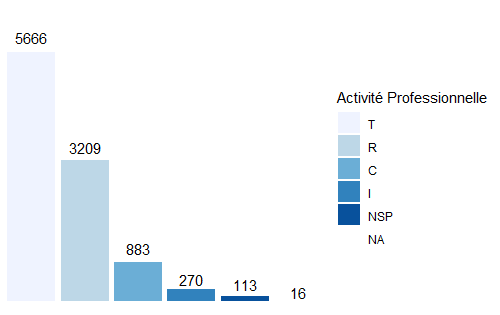
\includegraphics[scale=1]{activpro_barplot_manuel.png}
\end{center}

\noindent
Pour vérifier la cohérence des classes obtenues on peut tracer les distributions de l'âge dans chaque classe.\\

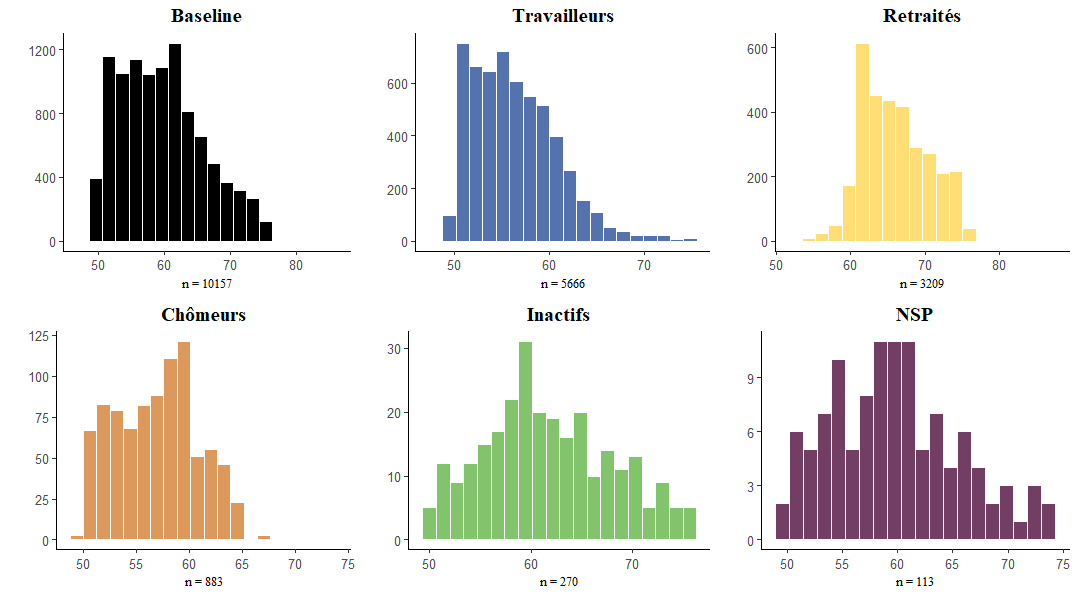
\includegraphics[scale=.5]{plot_grid_hist_age_activproBis.png}\\
\noindent
On remarque que 1116 sujets classés Travailleurs ont moins de 60 ans (on peut raisonnablement supposer que l'âge de la retraite est 60 ans car les sujets de la cohorte ont, à l'inclusion, un âge compris entre 50 et 75 ans).
De même, 134 sujets sont classés en tant que Retraités et ont moins de 60 ans.\\
\noindent
Ceci peut s'expliquer soit par une erreur de classification: ayant effectué cette dernière à la main il y a un risque non négligeable que je n'ai pas appliqué exactement le même critère de jugement pour chacun des cas. Il peut aussi ne pas s'agir d'une erreur, dans ce cas les données sont ainsi et on veillera simplement à garder cela à l'esprit lorsque nous interpréterons les résultats des tests statistiques ultérieurs.


\subsubsection{ACM et CAH}
\noindent
Pour vérifier la cohérence des résultats présentés au paragraphe précédent, j'ai effectué une Classification Ascendante Hiérarchique sur les résultats d'une Analyse des Correspondances Multiples appliquée
à une base de données constituée des quatre variables utilisées pour la classification "manuelle" : Adm12a, Adm11, Adm12 et Adm10. \\
J'ai également veillé à supprimer les individus (n = 29) ayant une valeur manquante pour l'une de ces quatre variables. \\

\noindent
Les résultats de l'ACM sont rassurants, dans le sens où l'emplacement dans le plan factoriel des quatre variables qui nous intéressent correspond à l'intuition qu'on en avait à savoir : 
\begin{itemize}
\item Les variables Adm12a et Adm11 apportent globalement la même information, cohérent puisque Adm12a et Adm11 discriminent les retraités et les travailleurs.
\item Adm12 et Adm10 sont sur le même plan horizontal : elles discriminent les chômeurs (avec les codes travail 91 à 96).
\item Adm12a, Adm10 sont dans le même plan vertical : elles discriminent les inactifs.
\end{itemize}
On s'attend donc à ce que la CAH effectuée sur les résultats de l'ACM produise une classification proche de celle effectuée à la main.\\
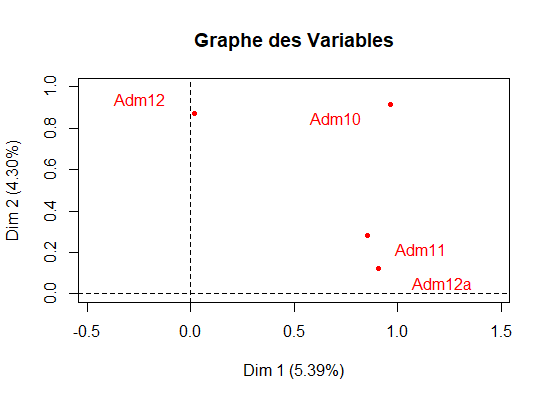
\includegraphics[scale = 1]{ACM_var.png}

\noindent
\textbf{NB:}Les faibles pourcentages d'inertie sont tout à fait normaux dans le cadre d'une ACM. En effet, comme l'explique Jérôme Pagès dans son livre "Analyse factorielle multiple avec R", si les variables étaient toutes identiques dans le cas d'une ACP la première dimension aurait 100\% d'inertie alors que dans une ACM la première dimension aurait au maximum $100\over{(nb_modalités - 1)}$ \% d'inertie.\\

\newpage
\noindent
Sur le graphe suivant on affiche les individus ainsi que les 15 modalités ayant la plus grande contribution. Ces 15 modalités sont affichées selon un gradient de couleur en fonction de leur $\cos^2$. \\

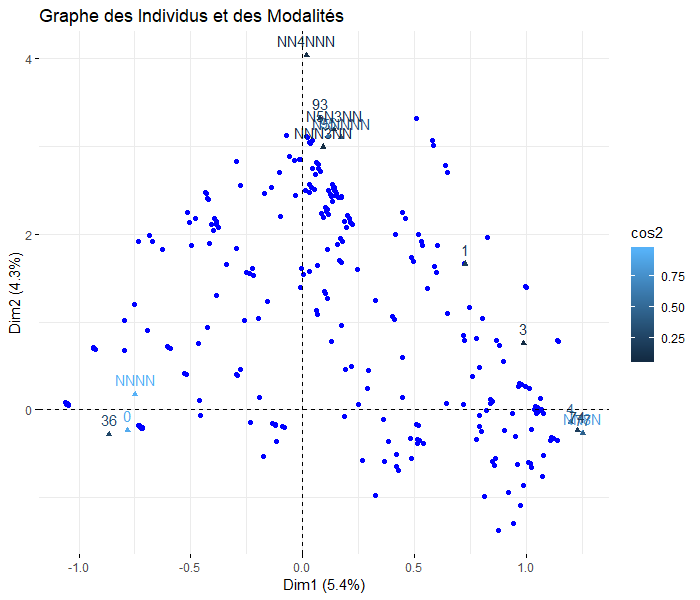
\includegraphics[scale = .4]{ACM_var_ind.png}\\

\noindent
On voit de façon assez claire trois groupes distincts : le premier en bas à droite est certainement celui des sujets retraités, on y retrouve les modalités 1,3,4 de Adm11 (ne travaille plus depuis resp, moin de 1 an, deux ans, trois ans et plus), 74 de Adm 10 (Ancien cadre), NN8N de Adm12a (Retraité).\\
\noindent
Le groupe en haut correspond sans doute aux chômeurs puisque les modalités NNN3NN, NN4NNN et N5N3NN de Adm12 (resp. A la recherche d'un emploi , Chômeur depuis moins de 6 mois et A la recherche d'un empois + Chômeur depuis 6 mois) et 93 de Adm10 (cadres et professions intellectuelles chômeurs).\\
Enfin le dernier groupe est celui en bas à gauche, il représente surement les travailleurs puisque la modalité 0 de Adm11 s'y trouve (Travaille) ainsi que 36 de Adm10 (Cadres) et NNNN de Adm12a. La présence de cette dernière modalité fait sens puisqu'elle représente les individus n'ayant rien coché dans la variable Adm12a doit les choix étaient pré-retraités, retraités, personne au foyer, en formation professionnelle. Or si ces sujets travaillent, aucune de ces catégories ne les concerne.\\

\noindent
Il reste deux choses qu'il me semble pertinent de relever: l'ACM semble particulièrement discriminer les cadres, on les retrouve dans les chômeurs, les retraités et les travailleurs. Ceci s'explique probablement par le fait que les modalités 36, 74 et 93 (resp Cadres d'entreprises, Anciens cadres et Cadres et professions intellectuelles chômeurs) représentent à elles seules 3848 sujets (sur 10157 sujets dans la base globale et 10128 dans la base ayant permis l'ACM).\\
La deuxième chose à noter est l'absence d'un quatrième groupe qui aurait représenté les inactifs. Une explication possible est la faible proportion de ces sujets dans la base. En effet lors de la classification manuelle on n'avait étiqueté "que" 270 sujets comme inactifs. \\

\noindent
La question que je me suis ensuite posée est celle de l'allure qu'aurait ma classification si elle était effectuée par un algorithme. De plus, il serait intéressant d'analyser la classification des individus que je n'ai pas su classer.
Pour cela j'ai effectué une Classification Ascendante Hiérarchique avec le package FactomineR de R en choisissant la distance du $\chi^2$ et le critère d'agrégation de Ward.\\

\noindent
\textbf{Distance du $\chi^2$ :}\\
\noindent
La distance entre un individu $i$ et un individus $j$ représentés par $p$ variables ayant $m_1$, $m_2$, $m_P$ modalités est donnée par:
\begin{center}
$d_{\chi^2}(i,j) = \sqrt{\sum_k{{np \over n_{.k}} {( {x_{ik}-x_{jk}\over p})^2}}}$
\end{center}
La distance du $\chi^2$ traduit le fait que deux individus ayant en commun une modalité rare sont plus proches que deux individus ayant en commun une modalité fréquente.\\

\noindent
\textbf{Méthode de Ward:}\\
C'est la méthode d'agrégation la plus courante. Elle consiste à choisir le réunion de deux groupes qui fera le moins baisser l'inertie entre les groupes, le but étant d'obtenir des groupes les plus "séparés" possible.\\


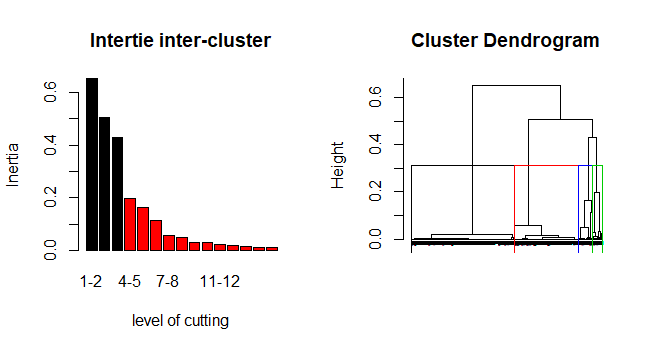
\includegraphics[scale = 1]{dendro_inertie_cah.png}
\noindent
Le graphe d'inertie semble indiquer que le nombre idéal de clusters est 4 ce qui est bon signe puisque l'idée était de répartir tous les sujets en 4 groupes : travailleurs, retraités, chômeurs et inactifs.\\

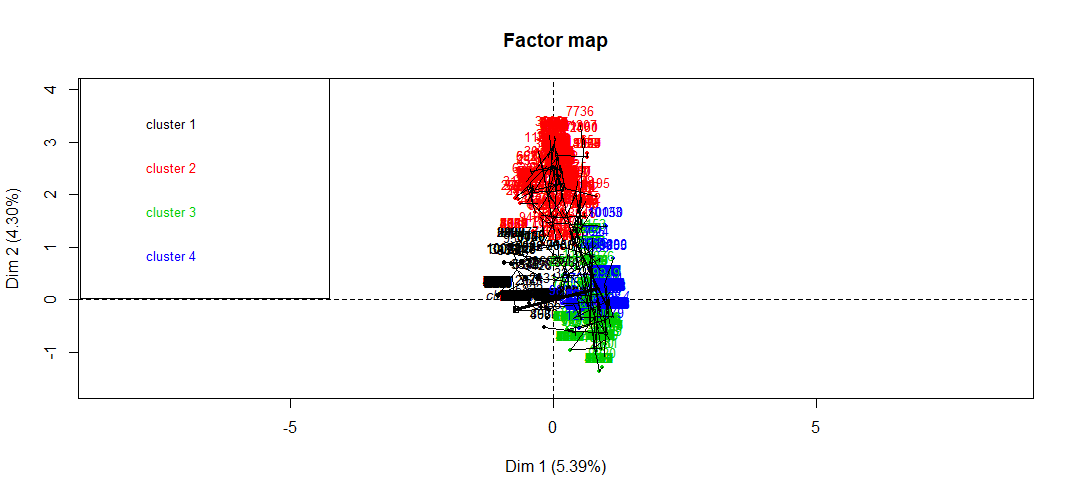
\includegraphics[scale = .5]{cah_ind_cluster.png}

\noindent
Pour pouvoir interpréter les Cluster obtenus par la CAH il est indispensable de comprendre quelles sont les modalités qui contribuent le plus à chaque Cluster.\\
Pour cela on cherche à déterminer si la forte présence d'une modalité dans un Cluster est due au hasard. Dans le cas contraire cela signifie que la modalité est représentative du Cluster.\\

\noindent
On effectue le test suivant pour chaque modalité dans chaque Cluster:\\
\noindent 
$H_0$ : La proportion de la modalité m dans le Cluster $c$ est due au hasard.\\
\noindent
$H_1$ : La proportion de la modalité m est anormalement élevée/basse dans le Cluster $c$.\\

\noindent
Ainsi sous $H_0$ on a :
\begin{center}
${{n_{mc}} \over {n_c}} = {{n_m} \over {n}}$
\end{center} 
où :\\
$n_{mc}$ est le nombre de sujet du Cluster $c$ présentant la modalité $m$,\\
$n_c$ est le nombre de sujets dans le Cluster $c$,\\
$n_m$ est le nombre de sujets présentant la modalité $m$,\\
$n$ est le nombre total d'individus.\\
	
\noindent
Sous $H_0$ : $n_{mc}  = {n_m . n_c \over {n}} $\\
Or le rapport ${n_m . n_c \over {n}} $ suit une loi hypergéométrique.\\
Soit $N_{mc}$ la variable aléatoire représentant le nombre d'individus de la modalité $m$ dans le Cluster $c$.
\begin{center}
$ N_{mc} \underset{H0}{\sim} \mathcal{H}(n, n_c, {{n_m}\over {m}})$
\end{center}

\noindent
La fonction catdes() du package FactoMineR nous résume les résultats de ce test pour chaque modalité dans chacun des Clusters en classant les modalités dans l'ordre décroissant de leur contribution au Cluster.
Seuls les test significatifs sont affichés.\\

\noindent
Dans les résultats affichés juste après, la première colonne correspond au nom de la modalité, la deuxième calcule le rapport $n_{mc} \over n_m$, la troisième le rapport $n_m \over n_c$, la quatrième le rapport $n_{mc} \over n$.\\
La cinquième colonne est le calcul de la p-valeur :\\
\begin{equation}
\mathbb{P}_{H0}(N_{mc} \geq n_{mc, obs}) =  \mathbb{P}_{\mathcal{H}(n, n_c, {n_m \over n})}(N_{mc} \geq n_{mc, obs})
\end{equation} 
Enfin, la dernière colonne est la valeur de la statistique de test calculée. Lorsqu'elle est positive la modalité à laquelle elle est associée est sur représentée dans le Cluster et lorsqu'elle est négative le modalité en question est sous représentée dans le Cluster.\\*

\noindent
Par souci de lisibilité nous n'afficheront que les modalités sur-représentées dans chaque Cluster:

\setlength\arrayrulewidth{2pt}
\arrayrulecolor{black}
\begin{tabular}{|c||ccccc|}
\hline
  \textbf{\textcolor{black}{Cluster 1}}       &    Cla/Mod  &   Mod/Cla   &   Global   &    p.value  &   v.test  \\
\hline
\hline 
            
Adm12a=NNNN  & 87.25 &99.91 &61.73  &0 &       Inf\\
Adm11=0      & 92.41 &99.29 &57.92  &0 &       Inf\\
Adm10=36     & 99.88 &46.21 &24.94  &0 &      Inf\\
Adm10=54     & 99.62 &14.41 & 7.80 &3.80e-217  &31.45\\
Adm12=NNNNNN & 57.94 &97.60 &90.82 &7.30e-155 & 26.51\\
Adm10=51     & 100 & 9.03 & 4.87 &1.12e-137  &24.98\\
Adm10=32     & 99.78 & 8.19 & 4.42 &3.78e-122  &23.50\\
Adm10=61     & 100 & 6.01 & 3.24 & 9.09e-91 & 20.20\\
Adm10=56     & 100 & 3.86 & 2.08 & 3.58e-58 & 16.08\\
Adm10=66     & 100 & 3.59 & 1.94 & 4.94e-54 & 15.48\\
Adm10=47     & 99.28 & 2.53 & 1.37 & 2.75e-36 & 12.58\\
Adm10=48    & 100 & 2.20 & 1.18 & 3.43e-33 & 12.00\\
Adm10=55    & 100& 1.41 & 0.76 & 1.70e-21 &  9.52\\
Adm12=6NNNNN & 80.52 & 2.27 & 1.52 & 4.19e-12  & 6.93\\
Adm10=41    & 100 & 0.77 & 0.41 & 4.99e-12 &  6.91\\
Adm10=46    & 100 &0.51 & 0.28 & 2.97e-08 &  5.54\\
\hline
\end{tabular}

\noindent
Les modalités de la variable Adm10 sur représentées dans le \textbf{\textcolor{black}{Cluster 1}} correspondent toutes à des codes travail de sujets qui travaillent. \\
La modalité la plus présente dans ce Cluster est Adm12a = NNNN, c'est à dire les sujets n'ayant coché aucune modalité de cette variable. Cela fait sens puisqu'aucune des modalités possibles ne traitaient d'une activité professionnelle. \\
Enfin les modalités de la variable Adm12 représentées dans le Cluster 1 sont NNNNNN c'est à dire ceux n'ayant rien coché et 6NNNNN : en contrat emplois-solidarité / intérim / CDD.\\


\bigskip
\setlength\arrayrulewidth{2pt}
\arrayrulecolor{red}
\begin{tabular}{|c||ccccc|}
\hline
 \textbf{\textcolor{red}{Cluster 2}}            &    Cla/Mod  &   Mod/Cla   &   Global   &    p.value  &   v.test  \\
\hline
\hline 
   
Adm12=N5NNNN  &99.74 &45.49 & 3.79 & 0   		&     Inf\\
Adm10=95      &98.52 &71.14 & 6.00 & 0  		&      Inf\\
Adm10=93      &100   &17.93 & 1.49 &1.42 e-169 	&27.76\\
Adm12=N5N3NN  &100   &17.81 & 1.48 &2.05 e-168  &27.66\\
Adm12a=NNNN   &12.59 &93.47 &61.73 &1.89 e-108  &22.12\\
Adm11=1       &37.58 &28.38 & 6.28 &1.39 e-103  &21.61\\
Adm12=NNN3NN  &90.65 &11.52 & 1.06 & 1.38 e-94  &20.63\\
Adm12=NN4NNN  & 100  &7.13 & 0.59 & 2.13 e-66  &17.21\\
Adm10=96      & 82.95 & 8.67 & 0.87 & 7.22 e-65  &17.01\\
Adm12=NN43NN& 100 & 4.99 & 0.41 & 1.65 e-46  &14.32\\
Adm12a=NNN7   &55.56 & 5.94 & 0.89 & 6.43 e-31  &11.56\\
Adm11=2       &26.68 &13.18 & 4.11 & 3.20 e-30  &11.42\\
Adm11=3       &24.17 &14.61 & 5.03  &5.04 e-29  &11.18\\
Adm10=94      &100 & 1.31 & 0.11  &1.23 e-12  & 7.10\\
Adm12=65NNNN  &78.57 & 1.31 & 0.14  &3.63 e-10  & 6.27\\
Adm12=6NN3NN  &70 & 0.83& 0.099  &2.66 e-06  & 4.70\\
Adm11=4       &10.34 & 32.54 &26.16  &1.61 e-05  & 4.31\\
Adm12=65N3NN  &100 & 0.48 & 0.04  &4.75 e-05  & 4.07\\
Adm12=6NNNNN & 17.53 & 3.21 & 1.52  &2.14 e-04  & 3.70\\
Adm12=6N43NN &100 & 0.36 & 0.03  &5.73 e-04  & 3.44\\
Adm12a=JNNN  & 66.67 & 0.24  &0.03  &2.01 e-02  & 2.32\\
\hline
\end{tabular}

\bigskip
\noindent
Dans le \textbf{\textcolor{red}{Cluster 2}}, les codes travail présents sont 94/93/94 : ils correspondent aux sujets chômeurs. De plus la modalité la plus représentée dans ce Cluster est Adm12 = N5NNNN : sujets chômeurs depuis plus de 6 mois.\\
Toutes les autres modalités de Adm12 présentent dans le Cluster concernent également des chômeurs.
Concernant la variable Adm11, les modalités présentes sont 1,2,3,4 c'est à dire les sujets ne travaillant plus depuis moins d'un an ou plus.\\
On remarque aussi que certains sujets en formation professionnelle (Adm12a = JNNN) sont inclus dans le Cluster.\\

\bigskip

\setlength\arrayrulewidth{2pt}
\arrayrulecolor{green}
\begin{tabular}{|c||ccccc|}
\hline
 \textbf{\textcolor{green}{Cluster 3}}   &    Cla/Mod  &   Mod/Cla   &   Global   &    p.value  &   v.test  \\
 \hline
 \hline
 Adm12a=N9NN &  99.41& 81.49 & 3.37 & 0.00 e+00    &    Inf\\
Adm10=85     & 98.25 &67.55  &2.82 & 0.00 e+00   &     Inf\\
Adm10=86     & 85.00 &28.61  &1.38 &3.76 e-149  &26.01\\
Adm11=5      & 94.23 &11.78  &0.51  &1.36 e-65  &17.10\\
Adm11=4      &  8.72 &55.53& 26.16  &2.07 e-38  &12.96\\
Adm12a=NNN7  & 36.67 & 7.93 & 0.89  &2.67 e-23  & 9.94\\
Adm12=NNNNNN &  4.47 &98.80 &90.82  &2.73 e-12  & 6.99\\
Adm12a=N9N7  &100.00  &1.68 & 0.07  &1.88 e-10  & 6.37\\
Adm12a=N98N  & 66.67 & 1.44 & 0.09  &3.57 e-07  & 5.09\\
\hline
\end{tabular} 

\bigskip

\noindent
Dans le \textbf{\textcolor{green}{Cluster 3}} la modalité la plus significativement représentée est Adm12a = N9NN : les personnes au foyer. On trouve également des sujet se déclarant en pré retraite (Adm12a = NNN7/N9N7 ou à la retraite(Adm12a = N98N).\\
Les seules modalités de la variables Adm10 dans ce cluster sont 85/86 ce qui semble indiquer que le Cluster correspond à celui des inactifs.\\
Enfin on remarque que plus de 94 \% des personnes déclarant n'avoir jamais travaillé sont dans le Cluster (Adm11 = 5).\\


\setlength\arrayrulewidth{2pt}
\arrayrulecolor{blue}
\begin{tabular}{|c||ccccc|}
\hline
   \textbf{\textcolor{blue}{Cluster 4}} &Cla/Mod  &   Mod/Cla      &Global      & p.value  &   v.test\\
   \hline
   \hline
Adm12a=NN8N &  99.09 &99.50 &33.81 & 0.00 e+00  &      Inf\\
Adm11=4      & 79.84 &62.02 &26.16 & 0.00 e+00  &      Inf\\
Adm10=77      &98.62 &62.73 &21.42 & 0.00 e+00  &      Inf\\
Adm10=74      &99.57 &34.19 &11.56 & 0.00 e+00  &      Inf\\
Adm12=NNNNNN  &36.99 &99.77 &90.82 &1.99 e-159  &26.90\\
Adm11=3       &72.89 &10.88 &5.06 & 7.49 e-77  &18.55\\
Adm11=2       &69.23 & 8.45 &4.11 & 1.43 e-51  &15.11\\
Adm11=1       &57.70 &10.76 &6.28 & 1.32 e-37  &12.82\\
Adm10=78     &100.00 & 2.05 &0.69 & 5.01 e-34  &12.16\\
Adm10=75     &100.00 & 0.79 &0.27  &1.60 e-13 &  7.38\\
\hline
\end{tabular}

\noindent
Enfin pour le \textbf{\textcolor{blue}{Cluster 4}} on s'attends à trouver des sujets retraités. En effet, la modalité la plus significativement représentée est Adm12a = NN8N : sujets retraités. \\
Les codes travail intervenant (variable Adm10) sont 77/74/78/75 : uniquement des codes de la forme "Ancien \textit{nom de la profession}".
En outre on ne trouve, dans ce Cluster, aucun individu déclarant travailler (Adm11 = 0 ou Adm12 = 6NNNNN).\\

\noindent
On peut alors conclure que  \textbf{le Cluster 1 correspond aux travailleurs}, \textbf{\textcolor{red}{le Cluster 2 aux chômeurs}}, \textbf{\textcolor{green}{le Cluster 3 aux inactifs}} et \textbf{\textcolor{blue}{le Cluster 4 aux retraités}}.

\subsubsection{Comparaisons des deux codages}
\noindent
Étudions les différences entre la classification manuelle et la Classification Ascendante Hiérarchique.\\
Tout d'abord on classe comme NA tous les sujets qui avaient une valeurs manquante pour au moins une des quatre variables ayant servies à la classification (n = 29).\\
On a alors : \\

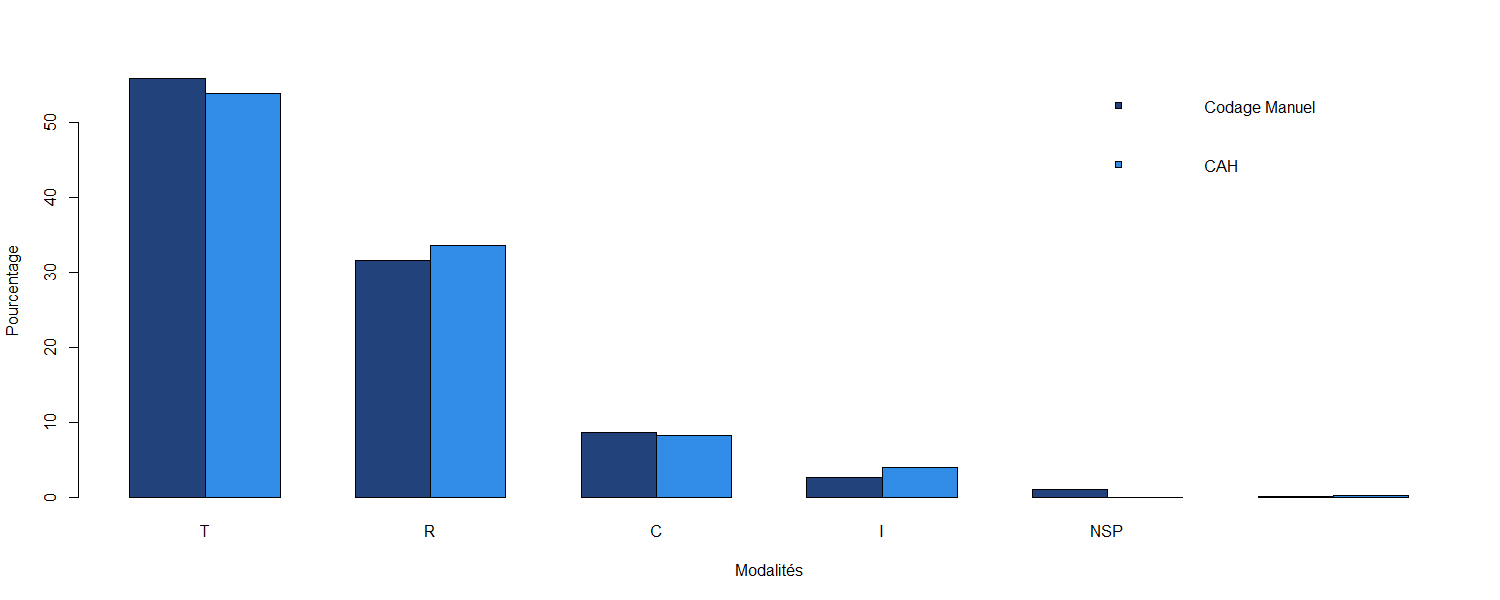
\includegraphics[scale=.4]{comp_codages_activpro_pourcentage.png}

\begin{center}
\setlength\arrayrulewidth{.5pt}
\arrayrulecolor{black}
\begin{tabular}{c|cccccc}

	& T & R & C & I & NSP & NA \\
	\hline
activpro & 5666 & 3209 & 883 & 270 & 113 & 16 \\
activproCAH	 & 5460 & 3410 &  842 & 416 & 0 & 29 \\
\hline
\hline
Différence & 206 & -201 &  41 & -146& 113& -13
\end{tabular}
\end{center}

\noindent
Il y a 509 sujets pour lesquels les deux classifications ne correspondent pas. Sur un total de 10157 cela représente 5,01 \% des sujets.\\
On remarque que la classification Ascendante Hiérarchique a tendance à classer plus facilement les sujets en Retraités et en Inactifs et la classification manuelle en Travailleurs. Une raison simple à cette différence est sans doute la volonté d'être le plus restrictifs possible quant à la classification manuelle des retraités.\\

\noindent
Le nombre de valeurs manquantes n'est pas le même pour les deux classifications pour une raison simple: les 16 NA de la classification manuelle sont des sujets pour lesquels TOUTES les variables nécessaires à la classification (Adm12a, Adm11, Adm12 et Am10) étaient manquantes alors que j'ai dû, pour la CAH, classer en NA les sujets pour lesquels AU MOINS UNE des 4 variables étaient manquantes afin de pouvoir réaliser l'ACM.\\

\noindent
Il peut également être intéressant d'étudier la manière dont les sujets classés NSP (n = 113) par la classification manuelle ont été classés par la CAH :\\

\begin{center}
\setlength\arrayrulewidth{.5pt}
\arrayrulecolor{black}
\begin{tabular}{|c|c|c|c||c|}
\hline
R & I & C & T & Total\\
\hline
5 & 77 & 0 & 31 & 113\\
\hline
\end{tabular}
\end{center}

\noindent
Sur quels critères la CAH s'est-elle basée pour classer ces 113 sujets ? 
Pour le comprendre on s'intéresse aux trois modalités dans lesquels elle a répartis les NSP (I,R,T) en construisant des Tableaux de Burt.\\

\noindent
Par souci de lisibilité j'ai choisis de n'inclure dans les tableaux de Burt que les modalités contenant un nombre de sujets non nul.\\
Les cases en rouge correspondent simplement aux tableaux de contingences usuels (croisement des variables deux à deux).\\
Le tableaux est évidement "symétrique", j'ai choisi de n'en remplir que la partie inférieure.\\


\begin{center} INACTIFS \end{center}

\begin{center}
\setlength\arrayrulewidth{.5pt}
\arrayrulecolor{green}
\begin{tabular}{|c|cc||cc||cc||ccc|}
\hline
	& N98N & N9NN & 0 & 4 & NNN3NN & NNNNN & 77 & 85 & 86\\
\hline
\hline
N98N & \textcolor{red}{1} &\textcolor{red}{$\emptyset$} & & & & & & & \\
N9NN &\textcolor{red}{$\emptyset$} & \textcolor{red}{76} & & & & & & & \\
\hline
\hline
0 & 0 & 76 & \textcolor{red}{76} & \textcolor{red}{$\emptyset$}& & & & & \\
4 & 1 & 0 &\textcolor{red}{$\emptyset$} & \textcolor{red}{1} & & & & &  \\
\hline
\hline
NNN3NN & 1 & 0 & 0 & 1 &\textcolor{red}{1} &\textcolor{red}{$\emptyset$} & & &  \\
\hline
NNNNNN & 0 & 76 & 76 &0 &\textcolor{red}{$\emptyset$} & \textcolor{red}{76} & & &\\
\hline
\hline
77 & 0 & 2 & 2 & 0 & 0 &2 & \textcolor{red}{2} &\textcolor{red}{$\emptyset$} &\textcolor{red}{$\emptyset$} \\
85/86 & 1 &74 & 74 & 1 & 1 & 74 &\textcolor{red}{$\emptyset$} & \textcolor{red}{58} & \textcolor{red}{17}\\
\hline
\end{tabular}
\end{center}

%\begin{center}
% Racine à Gauche, développement vers la droite
%\begin{tikzpicture}[xscale=.8,yscale=0.80]
% Styles (MODIFIABLES)
%\tikzstyle{fleche}=[->,>=latex,thick]
%\tikzstyle{noeud}=[fill=green!10,circle,minimum size = 1.5 cm, draw]
%\tikzstyle{feuille}=[fill=green!10 ,circle,draw, minimum size = 1.5 cm ]
%\tikzstyle{etiquette}=[midway,fill=white,draw]
%\tikzstyle{commentaire}=[right,black]
% Dimensions (MODIFIABLES)
%\def\DistanceInterNiveaux{3}
%\def\DistanceInterFeuilles{2}
% Dimensions calculées (NON MODIFIABLES)
%\def\NiveauA{(0)*\DistanceInterNiveaux}
%\def\NiveauB{(1.6666666666666665)*\DistanceInterNiveaux}
%\def\NiveauC{(3)*\DistanceInterNiveaux}
%\def\NiveauD{(4)*\DistanceInterNiveaux}
%\def\InterFeuilles{(-1)*\DistanceInterFeuilles}
% Noeuds (MODIFIABLES : Styles et Coefficients d'InterFeuilles)
%\node[noeud] (R) at ({\NiveauA},{(2.5)*\InterFeuilles}) {$Inactifs$};
%\node[noeud] (Ra) at ({\NiveauB},{(1)*\InterFeuilles}) {$N98N$};
%\node[feuille] (Raa) at ({\NiveauC},{(0)*\InterFeuilles}) {$0$};
%\draw (Raa.east) node[commentaire] {$$};
%\node[noeud] (Rab) at ({\NiveauC},{(1.5)*\InterFeuilles}) {$4$};
%\node[feuille] (Raba) at ({\NiveauD},{(1)*\InterFeuilles}) {$77$};
%\draw (Raba.east) node[commentaire] {$$};
%\node[feuille] (Rabb) at ({\NiveauD},{(2)*\InterFeuilles}) {$85/86$};
%\draw (Rabb.east) node[commentaire] {$1$};
%\node[noeud] (Rb) at ({\NiveauB},{(4)*\InterFeuilles}) {$N9NN$};
%\node[noeud] (Rba) at ({\NiveauC},{(3.5)*\InterFeuilles}) {$0$};
%\node[feuille] (Rbaa) at ({\NiveauD},{(3)*\InterFeuilles}) {$77$};
%\draw (Rbaa.east) node[commentaire] {$2$};
%\node[feuille] (Rbab) at ({\NiveauD},{(4)*\InterFeuilles}) {$85/86$};
%\draw (Rbab.east) node[commentaire] {$3$};
%\node[feuille] (Rbb) at ({\NiveauC},{(5)*\InterFeuilles}) {$4$};
%\draw (Rbb.east) node[commentaire] {$$};
% Arcs (MODIFIABLES : Styles)
%\draw[fleche] (R)--(Ra) node[etiquette] {$1$};
%\draw[fleche] (Ra)--(Raa) node[etiquette] {$0$};
%\draw[fleche] (Ra)--(Rab) node[etiquette] {$1$};
%\draw[fleche] (Rab)--(Raba) node[etiquette] {$0$};
%\draw[fleche] (Rab)--(Rabb) node[etiquette] {$1$};
%\draw[fleche] (R)--(Rb) node[etiquette] {$76$};
%\draw[fleche] (Rb)--(Rba) node[etiquette] {$76$};
%\draw[fleche] (Rba)--(Rbaa) node[etiquette] {$2$};
%\draw[fleche] (Rba)--(Rbab) node[etiquette] {$74$};
%\draw[fleche] (Rb)--(Rbb) node[etiquette] {$0$};
%\end{tikzpicture}
%\end{center}
\bigskip

\noindent
1 sujet déclare être au foyer et à la retraite (Adm12a = "N98N), ne plus tavailler depuis au moins 3 ans (Adm11 = 4) et a un code travail correspondant à un inactif non retraité (Adm10 + 85/86). Le classer en Inactifs a donc du sens. \\

\noindent
2 sujets déclarent être au foyer (Adm12a = N9NN), travailler (Adm11 = 0) et ont un code travail correspondant à un retraité (Adm10 = 77 : Ancien employé). Toutes les variables sont contradictoires. Classer ces sujets en Inactifs n'est pas pertinent.\\

\noindent
74 sujets présentent les même caractéristiques que ceux expliqués précédemment à l'exception de la variable Adm10 qui indique que les sujets sont inactifs non retraités. De même, les classer en inactifs n'est pas pertinent.\\

\noindent
De manière générale on remarque que déclarer être "au foyer" est très discriminant pour la classification en tant qu'inactifs surtout si cette modalité est couplée avec un code travail 85 ou 86.\\


\begin{center} RETRAITES \end{center}

\begin{center}
\setlength\arrayrulewidth{.5pt}
\arrayrulecolor{blue}
\begin{tabular}{|c||ccc||cc||c||c||c|}
\hline
 &N98N &NN87& NN8N& 0& 4& NNNNNN& 32/36& 77\\
 \hline
 \hline
 N98N &\textcolor{red}{1}& \textcolor{red}{$\emptyset$}& \textcolor{red}{$\emptyset$} & & & & & \\
NN87 & \textcolor{red}{$\emptyset$} & \textcolor{red}{1} &\textcolor{red}{$\emptyset$}& & & & & \\
NN8N & \textcolor{red}{$\emptyset$} & \textcolor{red}{$\emptyset$} & \textcolor{red}{3} & & & & & \\
\hline
\hline
0 & 1 & 1 & 0 & \textcolor{red}{2} & \textcolor{red}{$\emptyset$} &&&\\
4 & 0 & 0 & 3 & \textcolor{red}{$\emptyset$} & \textcolor{red}{3} &&&\\
\hline
\hline
NNNNNN & 1 & 1 & 3 & 2 & 3 & \textcolor{red}{5} & & \\
\hline
\hline
32/36 & 0 & 0 & 3 & 0 3 &3 & \textcolor{red}{1} & \textcolor{red}{2} & \textcolor{red}{$\emptyset$}\\
\hline
\hline
77 & 1 & 1 & 0 & 2 & 0 & 2 & \textcolor{red}{$\emptyset$} & \textcolor{red}{2}\\
\hline
\end{tabular}
\end{center}
% Racine à Gauche, développement vers la droite
%\begin{tikzpicture}[xscale=.7,yscale=.8]
% Styles (MODIFIABLES)
%\tikzstyle{fleche}=[->,>=latex,thick]
%\tikzstyle{noeud}=[fill=blue!10,circle,minimum size = 1.5 cm, draw]
%\tikzstyle{feuille}=[fill=blue!10,circle,minimum size = 1.5 cm, draw]
%\tikzstyle{etiquette}=[midway,fill=white,draw]
%\tikzstyle{commentaire}=[right,black]
% Dimensions (MODIFIABLES)
%\def\DistanceInterNiveaux{3}
%\def\DistanceInterFeuilles{2}
% Dimensions calculées (NON MODIFIABLES)
%\def\NiveauA{(0)*\DistanceInterNiveaux}
%\def\NiveauB{(1.6666666666666665)*\DistanceInterNiveaux}
%\def\NiveauC{(3)*\DistanceInterNiveaux}
%\def\NiveauD{(4)*\DistanceInterNiveaux}
%\def\InterFeuilles{(-1)*\DistanceInterFeuilles}
% Noeuds (MODIFIABLES : Styles et Coefficients d'InterFeuilles)
%\node[noeud] (R) at ({\NiveauA},{(4)*\InterFeuilles}) {$Retraites$};
%\node[noeud] (Ra) at ({\NiveauB},{(1)*\InterFeuilles}) {$N98N$};
%\node[noeud] (Raa) at ({\NiveauC},{(0.5)*\InterFeuilles}) {$0$};
%\node[feuille] (Raaa) at ({\NiveauD},{(0)*\InterFeuilles}) {$77$};
%\draw (Raaa.east) node[commentaire] {$1$};
%\node[feuille] (Raab) at ({\NiveauD},{(1)*\InterFeuilles}) {$32/36$};
%\draw (Raab.east) node[commentaire] {$$};
%\node[feuille] (Rab) at ({\NiveauC},{(2)*\InterFeuilles}) {$4$};
%\draw (Rab.east) node[commentaire] {$$};
%\node[noeud] (Rb) at ({\NiveauB},{(4)*\InterFeuilles}) {$NN8N$};
%\node[feuille] (Rba) at ({\NiveauC},{(3)*\InterFeuilles}) {$0$};
%\draw (Rba.east) node[commentaire] {$$};
%\node[noeud] (Rbb) at ({\NiveauC},{(4.5)*\InterFeuilles}) {$4$};
%\node[feuille] (Rbba) at ({\NiveauD},{(4)*\InterFeuilles}) {$77$};
%\draw (Rbba.east) node[commentaire] {$$};
%\node[feuille] (Rbbb) at ({\NiveauD},{(5)*\InterFeuilles}) {$32/36$};
%\draw (Rbbb.east) node[commentaire] {$2$};
%\node[noeud] (Rc) at ({\NiveauB},{(7)*\InterFeuilles}) {$NN87$};
%\node[noeud] (Rca) at ({\NiveauC},{(6.5)*\InterFeuilles}) {$0$};
%\node[feuille] (Rcaa) at ({\NiveauD},{(6)*\InterFeuilles}) {$77$};
%\draw (Rcaa.east) node[commentaire] {$3$};
%\node[feuille] (Rcab) at ({\NiveauD},{(7)*\InterFeuilles}) {$32/36$};
%\draw (Rcab.east) node[commentaire] {$$};
%\node[feuille] (Rcb) at ({\NiveauC},{(8)*\InterFeuilles}) {$4$};
%\draw (Rcb.east) node[commentaire] {$$};
% Arcs (MODIFIABLES : Styles)
%\draw[fleche] (R)--(Ra) node[etiquette] {$1$};
%\draw[fleche] (Ra)--(Raa) node[etiquette] {$1$};
%\draw[fleche] (Raa)--(Raaa) node[etiquette] {$1$};
%\draw[fleche] (Raa)--(Raab) node[etiquette] {$0$};
%\draw[fleche] (Ra)--(Rab) node[etiquette] {$0$};
%\draw[fleche] (R)--(Rb) node[etiquette] {$3$};
%\draw[fleche] (Rb)--(Rba) node[etiquette] {$0$};
%\draw[fleche] (Rb)--(Rbb) node[etiquette] {$3$};
%\draw[fleche] (Rbb)--(Rbba) node[etiquette] {$0$};
%\draw[fleche] (Rbb)--(Rbbb) node[etiquette] {$3$};
%\draw[fleche] (R)--(Rc) node[etiquette] {$1$};
%\draw[fleche] (Rc)--(Rca) node[etiquette] {$1$};
%\draw[fleche] (Rca)--(Rcaa) node[etiquette] {$1$};
%\draw[fleche] (Rca)--(Rcab) node[etiquette] {$0$};
%\draw[fleche] (Rc)--(Rcb) node[etiquette] {$0$};
%\end{tikzpicture}

\bigskip

\noindent
1 déclare être à la retraite et au foyer (N98N) avec un code de travail correspondant bien à un retraité (77). Cependant il déclare également travailler (0). La CAH le classe en retraité malgré tout mais ce choix n'est pas judicieux.\\

\noindent
3 sujets se déclarent à la retraite (NN8N), ne travaillant plus (Adm11 = 3) et ont un code travail qui correspond à des travailleurs (Adm10 = 32/36). Leur classification en Retraité n'est pas aberrante. Il est possible que ces sujets n'aient pas lu la liste des codes travail jusqu'à la fin (la où ceux concernant les retraités se trouvent) ce qui expliquerait qu'ils aient indiqué par ce code qu'ils travaillent (32/36).\\

\noindent
1 sujet déclare être retraité et pré-retraité (NN87), travailler (Adm11 = 0) et a un code travaille de 77. Il y a une certaine forme de cohérence à l'ensemble des choix de ce sujet mais on ne peux pas le classer en tant que Retraité à cause de Adm11 = 0. 


\begin{center}TRAVAILLEURS\end{center}
\begin{center}
\setlength\arrayrulewidth{.6pt}
\arrayrulecolor{black}
\begin{tabular}{|c||cc||cccc||c||ccc|}
\hline
 & NNN7 & NNNN & 0 & 1 & 3 & 4 & NNNNNN & \begin{tabular}{c}
32/36/47/48/  \\
 51/54/55/56
\end{tabular} & 85/86 & 88 \\
 \hline
 \hline
NNN7 & \textcolor{red}{1} & \textcolor{red}{$\emptyset$}& & & & & & & & \\
NNNN & \textcolor{red}{$\emptyset$} &\textcolor{red}{30} & & & & & & &  &\\
\hline
\hline
0 & 0 & 12 & \textcolor{red}{12} & \textcolor{red}{$\emptyset$} & \textcolor{red}{$\emptyset$} & \textcolor{red}{$\emptyset$} & & & &  \\
1 & 0 & 1 & \textcolor{red}{$\emptyset$} & \textcolor{red}{1} & \textcolor{red}{$\emptyset$} & \textcolor{red}{$\emptyset$} & & & &  \\
3 & 0 & 1 & \textcolor{red}{$\emptyset$} & \textcolor{red}{$\emptyset$} & \textcolor{red}{1} & \textcolor{red}{$\emptyset$} & & & &  \\
4 & 1 & 16 & \textcolor{red}{$\emptyset$} & \textcolor{red}{$\emptyset$} & \textcolor{red}{$\emptyset$} & \textcolor{red}{17}& & & & \\
\hline
\hline
NNNNNN & 1 & 30 & 12 & 1  & 1 & 171 & \textcolor{red}{31} & &  &\\
\hline
\hline
\begin{tabular}{c}
32/36/47/48/  \\
 51/54/55/56
\end{tabular}
 & 1 & 18 & 0 & 1 & 1 & 17 & 19 & \textcolor{red}{19} & \textcolor{red}{$\emptyset$} & \textcolor{red}{$\emptyset$}\\
 85/86 & 0 & 11 & 11 & 0 & 0 & 0 & 11 & \textcolor{red}{$\emptyset$} & \textcolor{red}{11} & \textcolor{red}{$\emptyset$}\\
 \hline
 88 & 0 & 1 & 1 & 0 & 0 & 0 & 1 & \textcolor{red}{$\emptyset$} & \textcolor{red}{$\emptyset$} & \textcolor{red}{1}\\
 \hline
\end{tabular}
\end{center}


%:-+-+-+- Engendré par : http://math.et.info.free.fr/TikZ/Arbre/
%\begin{center}
% Racine à Gauche, développement vers la droite
%\begin{tikzpicture}[xscale=.7,yscale=.76]
% Styles (MODIFIABLES)
%\tikzstyle{fleche}=[->,>=latex,thick]
%\tikzstyle{noeud}=[fill=black!15,circle, minimum size = 1.5 cm , draw]
%\tikzstyle{feuille}=[fill=black!15,circle ,minimum size = 1.5 cm, draw]
%\tikzstyle{etiquette}=[midway,fill=white,draw]
%\tikzstyle{commentaire}=[right,black]
% Dimensions (MODIFIABLES)
%\def\DistanceInterNiveaux{3}
%\def\DistanceInterFeuilles{2}
% Dimensions calculées (NON MODIFIABLES)
%\def\NiveauA{(0)*\DistanceInterNiveaux}
%\def\NiveauB{(1.6666666666666665)*\DistanceInterNiveaux}
%\def\NiveauC{(3)*\DistanceInterNiveaux}
%\def\NiveauD{(4)*\DistanceInterNiveaux}
%\def\InterFeuilles{(-1)*\DistanceInterFeuilles}
% Noeuds (MODIFIABLES : Styles et Coefficients d'InterFeuilles)
%\node[noeud] (R) at ({\NiveauA},{(4.5)*\InterFeuilles}) {$Travailleurs$};
%\node[noeud] (Ra) at ({\NiveauB},{(1.5)*\InterFeuilles}) {$NNN7$};
%\node[feuille] (Raa) at ({\NiveauC},{(0)*\InterFeuilles}) {$0$};
%\draw (Raa.east) node[commentaire] {$$};
%\node[noeud] (Rab) at ({\NiveauC},{(2)*\InterFeuilles}) {$1/3/4$};
%\node[feuille] (Raba) at ({\NiveauD},{(1)*\InterFeuilles}) {$85/86$};
%\draw (Raba.east) node[commentaire] {$$};
%\node[feuille] (Rabb) at ({\NiveauD},{(2)*\InterFeuilles}) {$88$};
%\draw (Rabb.east) node[commentaire] {$$};
%\node[feuille] (Rabc) at ({\NiveauD},{(3)*\InterFeuilles}) {$Reste$};
%\draw (Rabc.east) node[commentaire] {$1$};
%\node[noeud] (Rb) at ({\NiveauB},{(6.5)*\InterFeuilles}) {$NNNN$};
%\node[noeud] (Rba) at ({\NiveauC},{(5)*\InterFeuilles}) {$0$};
%\node[feuille] (Rbaa) at ({\NiveauD},{(4)*\InterFeuilles}) {$85/86$};
%\draw (Rbaa.east) node[commentaire] {$2$};
%\node[feuille] (Rbab) at ({\NiveauD},{(5)*\InterFeuilles}) {$88$};
%\draw (Rbab.east) node[commentaire] {$3$};
%\node[feuille] (Rbac) at ({\NiveauD},{(6)*\InterFeuilles}) {$Reste$};
%\draw (Rbac.east) node[commentaire] {$$};
%\node[noeud] (Rbb) at ({\NiveauC},{(8)*\InterFeuilles}) {$1/3/4$};
%\node[feuille] (Rbba) at ({\NiveauD},{(7)*\InterFeuilles}) {$85/86$};
%\draw (Rbba.east) node[commentaire] {$$};
%\node[feuille] (Rbbb) at ({\NiveauD},{(8)*\InterFeuilles}) {$88$};
%\draw (Rbbb.east) node[commentaire] {$$};
%\node[feuille] (Rbbc) at ({\NiveauD},{(9)*\InterFeuilles}) {$Reste$};
%\draw (Rbbc.east) node[commentaire] {$4$};
% Arcs (MODIFIABLES : Styles)
%\draw[fleche] (R)--(Ra) node[etiquette] {$1$};
%\draw[fleche] (Ra)--(Raa) node[etiquette] {$0$};
%\draw[fleche] (Ra)--(Rab) node[etiquette] {$1$};
%\draw[fleche] (Rab)--(Raba) node[etiquette] {$0$};
%\draw[fleche] (Rab)--(Rabb) node[etiquette] {$0$};
%\draw[fleche] (Rab)--(Rabc) node[etiquette] {$1$};
%\draw[fleche] (R)--(Rb) node[etiquette] {$30$};
%\draw[fleche] (Rb)--(Rba) node[etiquette] {$12$};
%\draw[fleche] (Rba)--(Rbaa) node[etiquette] {$11$};
%\draw[fleche] (Rba)--(Rbab) node[etiquette] {$1$};
%\draw[fleche] (Rba)--(Rbac) node[etiquette] {$0$};
%\draw[fleche] (Rb)--(Rbb) node[etiquette] {$18$};
%\draw[fleche] (Rbb)--(Rbba) node[etiquette] {$0$};
%\draw[fleche] (Rbb)--(Rbbb) node[etiquette] {$0$};
%\draw[fleche] (Rbb)--(Rbbc) node[etiquette] {$18$};
%\end{tikzpicture}
%\end{center}
%:-+-+-+-+- Fin
\bigskip

\noindent
1 sujet se déclare pré-retraité (NNN7), travaille (Adl11 = 0) et a un code travail correspondant à quelqu'un ayant encore une activité professionnelle. On peut accepter la classification en travailleur de ce sujet par la CAH.\\

\noindent
11 sujets ne cochent aucune case pour Adm12a (soit ils ont oublié cette question soit aucun des choix ne les satisfont ce qui correspondrait à des personnes qui travaillent puisque ce choix n'est pas proposé dans Adm12a).En outre ils déclarent travailler (Adm11 = 0) mais leur code travail est incohérent: 85/86 correspond à des inactifs.\\

\noindent
1 sujet travaille et a un code travail qui vaut 88. Ce code n'est pas présent dans la liste, il s'agit probablement d'une faute de frappe.\\

\noindent
Enfin, 18 sujets déclarent ne plus travailler (Adm11 = 1/3/4)mais ont un code travail indiquant qu'ils ont encore une activité professionnelle. Ces sujets ne peuvent pas être classés comme des travailleurs.\\

\noindent
A présent que les deux classifications sont établies et clairement expliquées, il y a lieu de se demander si utiliser l'une ou l'autre dans un futur modèle changera les résultats.\\
Autrement dit construisons un test permettant de vérifier si les deux distributions de la variable activité professionnelle sont similaires.\\

\noindent
\textbf{Test du Khi deux d'ajustement}\\
Il s'agit de vérifier si les écarts d'effectifs entre le codage manuel et la CAH sont "trop" importants pour chacune des classes.\\
Étant donné que la CAH classe TOUS les individus, la classe NSP de la CAH est vide.
Or le test du $\chi^2$ d'ajustement n'est applicable que si toutes les classes contiennent au moins 5 sujets.\\
Puisque nous nous intéressons particulièrement aux Travailleurs, Retraités et Chômeurs, on rassemble les inactifs, les NSP et les NA dans une classe "AUTRE".\\
\noindent
On a alors:\\

\begin{center}
\setlength\arrayrulewidth{.1pt}
\arrayrulecolor{black}
\begin{tabular}{|c||c|c|c|c|}
\hline
	& T & R & C & Autre\\
\hline
\hline
activpro & 5666 & 3209 & 883 & 299\\
\hline
activproCAH & 5460 & 3410 & 842 & 445\\
\hline
\end{tabular}
\end{center}
\noindent
Notations : \\
$k$ : nombre de modalités.\\
$\phi_i$ : probabilité qu'un individus soit dans la classe $i$ de la distribution observée.\\ 
$\phi_{hi}$ : probabilité qu'un individu soit dans la classe $i$ de la distribution théorique.\\
$O_i$ : nombre d'individus observés dans la modalité $i$.\\
$A_i$ : nombre d'individus attendus dans la modalité $i$.\\
On a : $\forall i \in \ldbrack 1,k \rdbrack , A_i = n \phi_{hi}$\\

\noindent
Hypothéses :
\begin{align*}
H_0 : \forall i \in \ldbrack 1,k \rdbrack ,\phi_i = \phi_{hi}\\
H_1 : \exists i \in \ldbrack 1,k \rdbrack tq \phi_i \neq \phi_{hi}
\end{align*}

\noindent
Statistique de test:
\begin{center}
$Q = \sum_{i=1}^k ~{{(O_i - A _i)^2} \over {A_i}}$
\end{center}

\noindent
D'après le Théorème de Pearson : 

\begin{align*}
Si ~\forall i  \in \ldbrack 1,k \rdbrack, ~ A_i \geq 5 :\\
Q \underset {\small{H_0}}{\hookrightarrow} \chi ^{2} (k-1) , ~ n \rightarrow +\infty
\end{align*}


\noindent
\textbf{Application numérique:} \\
\noindent
 $Q_{obs} = 69.52$ 
Au niveau de confiance 95 \% le $\chi ^2$ à 3 degrés de liberté vaux 12.84.\\
On rejette donc $H_0$.
\\
\noindent
On ne peut pas conclure que les deux variables ont une distribution similaire. Cependant après avoir observé la manière dont les sujets "inclassables" ont été classés par la CAH il semble préférable de se baser sur la classification manuelle de l'activité professionnelle des sujets de l'étude. En analyse de sensibilité nous feront tourner le modèle final sur les données classifiées par la machine.\\
\subsection{Variable d'intérêt : Self Rated Health (SRH)}
\noindent
La santé perçue est décrite dans la littérature comme un bon indicateur de la mortalité. Il s'agit d'une mesure subjective puisque le sujet s'auto-évalue : il est son propre témoin.\\
Dans le questionnaire d'inclusion il est demandé aux sujets d'indiquer par une note comprise entre 0 et 10 leur état de santé tel qu'il le ressente: 0 pour mauvais et 10 pour excellent.\\
\noindent
Globalement les sujets de la cohorte EPP3 s'estiment en bonne santé avec une médiane à 7.\\ En choisissant ce cut off on crée une variable binaire de santé perçue:

\begin{center}

\setlength\arrayrulewidth{.1pt}
\arrayrulecolor{black}
\begin{tabular}{|c|c|c|}
\hline
  0  &  1& NA \\
  \hline
  \hline 
4390& 5741&   26\\
\hline 
\end{tabular}
%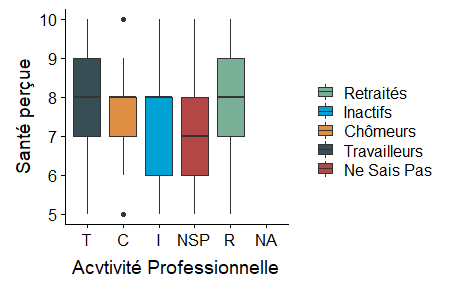
\includegraphics[scale=.5]{activpro_srh_boxplot.png}
\end{center}

\noindent
\textbf{Test du $\chi^2$ d'indépendance entre la santé perçue et l'activité professionnel des sujets de la cohorte EPP3.}\\

\noindent
On note:\\

\noindent
$X$ la v.a qualitative à $l$ modalités.\\
$Y$ le v.a qualitative à $c$ modalités.\\

\noindent
$\forall (i,j) \in \ldbrack 0,5 \rdbrack \times \ldbrack 0,11 \rdbrack$ :\\
$n_{i,j}$ = Nombre de sujets présentant la modalité $i$ de la variable $X$ et la modalité $j$ de la variable $Y$.\\
$n_{i.} = \sum_{j = 1} ^c n_{ij}$ : nb total individus dans la classe $i$ de la v.a $X$.\\
$n_{.j} = \sum_{i = 1} ^l n_{ij}$ : nb total d'individus dans la classe $j$ de la v.a $Y$.\\
\noindent
$n = \sum _{i = 1} ^ l \sum_{j = 1} ^c n_{ij}$ : nb total d'individus.\\

\noindent
On teste $H_0 : X \perp Y $ contre $H_1 = \overline{H_0}$\\

\noindent
Statistique de test : 
\begin{align*}
Q = {\sum _{i = 1} ^l \sum_{j = 1} ^c {{(n_{ij} - {{n_{i.}.n_{.j}}\over{n}})^2}} \over {{n_{i.}.n_{.j}}\over{n}}}
\end{align*}

\noindent
On a : \\
\begin{align*}
Q \underset {\small{H_0}}{\large{\sim}} \chi ^{2} ((l-1)(c-1))
\end{align*}
\noindent
On pose :\\
\begin{align*}
e_{ij} = { {n_{i.}.n_ {.j} } \over {n} }
\end{align*}
C'est l'effectif théorique sous $H_0$ c'est à dire le nombre de sujets présentant les modalités i et j (resp. des v.a X et Y) auxquelles on s'attend sous $H_0$.\\

\noindent
Règle de décision :\\
Si $Q_{calc} \geq Q_{th}$ on rejette $H_0$ (où $Q_{th}$ est le quantile de la loi du $\chi ^2$ à $(l-1)(c-1)$ degrés de libertés pour un niveau de confiance $\alpha$ fixé).\\

\noindent
Le test du $\chi ^2$ d'indépendance n'est applicable que lorsque $\forall (i,j) \in \ldbrack 1,l \rdbrack \times \ldbrack 1,c \rdbrack : e_{ij} \geq 5 ~et ~n_{ij} \geq 50.$\\

\noindent
Application numérique:\\
Le tableau de contingence des variables activpro et srh présente des cases dont les effectifs sont inférieurs à 5. Pour effectuer le test on se base donc sur la version binarisée de la variable de santé perçue.\\

\noindent
On pose :\\
\noindent
$X$ v.a qualitative à 11 modalités représentant la santé perçue des sujets.\\
\noindent
$Y$ v.a qualitative à 5 modalités représentant l'activité professionnelle des sujets.\\

\noindent
On trouve $Q_{calc} = 31.71$ et $\chi ^2 _ {4 ~dll, \alpha = 5 \%} = 9.49$ donc on rejette $H_0$ avec une \textbf{p-valeur de $2.19 ~10^{-6}$}.\\
Autrement dit il existe un lien fort entre l'activité professionnelle et la santé perçue des sujets de la cohorte EPP3.\\
\noindent
Lorsque l'on fait le test avec la variable activproCAH plutôt que activpro (en retirant la classe NSP puisqu'elle est évidement vide) on obtient également une p-valeur significative ($Q_{calc} = 21.51$, $Q_{th} = 7.81$ et $p= 8.24 ~10^{-6}$).

\subsection{Variables d'ajustement et facteurs de confusion}
\noindent
Rappelons qu'un facteur de confusion est une variable à la fois liée à l'exposition et à la variable d'intérêt.
Notre variable d'exposition est l'activité professionnelle des sujets et la variable d'intérêt leur santé perçue.\\

\noindent
Le facteur de confusion le plus évident est donc l'âge du sujet puisque celui ci est determinant dans l'exercice d'une activité professionnelle mais joue également un rôle dans la perception qu'ont les sujets de leur santé.\\

\noindent
Les autres variables d'ajustement sont choisies en se basant sur la littérature : sexe, alcool, tabac, score de dépression, statut marital, indice de masse corporel, diabète, activité sportive et niveau d'éducation.\\


\noindent
Rappelons que l'indice de masse corporel est le rapport entre le poids et la taille carrée des individus. \\


\noindent
Le score de dépression est quant à lui la somme de 13 variables binaires :
\baselineskip 1pt
\begin{enumerate}
\item En ce moment ma vie me semble vide.
\item J'ai du mal à me débarrasser des mauvaises pensées qui me passent par la tête.
\item Je suis sans énergie.
\item Je me sens bloqué(e) ou empêché(e) devant la moindre chose à faire.
\item Je suis déçu(e) et dégouté(e) de moi-même.
\item Je suis obligé(e) de me forcer pour faire quoi que ce soit.
\item J'ai du mal à faire les choses que j'avais l'habitude de faire.
\item En ce moment je suis triste.
\item J'ai l'esprit moins clair que d'habitude.
\item J'aime moins qu'avant faire les choses qi me plaisent ou m'intéressent.
\item Ma mémoire me semble moins bonne que d'habitude.
\item Je suis sans espoir pour l'avenir.
\item En ce moment je me sens moins heureux(se) que la plupart des gens.
\end{enumerate}

\noindent
On considère qu'un sujet est déprimé si son score de dépression est supérieur ou égal à 7 ou s'il déclare prendre des antidépresseurs.\\

\smallskip

\noindent
J'ai également choisi d'ajouter quelques autres variables qui m'ont semblé pertinentes: maladie indice de précarité (EPICE) de vie et score de stress (PSS4) qui sont deux indicateurs trés utilisés en épidémiologie et que de nombreuses études ont jugés consistants \cite{warttig_new_2013} \cite{sass_comparaison_2006}.

\bigskip
\noindent
Le score EPICE est un score Évaluant de la Précarité et des Inégalités de santé dans les Centres d'Examens
de santé) prenant en compte diverses informations :
\begin{enumerate}
\item Rencontrez-vous parfois un travailleur social (assistante sociale, éducateur) ?\\
coeff = 10,06
\item Bénéficiez-vous d'une assurance maladie complémentaire (mutuelle) coeff = -11,83
\item Vivez-vous en couple ? coeff = -8,28
\item Etes-vous propriétaire de votre logement (ou accédant à la propriété) ?\\
coeff = -8,28
\item Y-a-t-il des périodes dans le mois où vous rencontrez de réelles difficultés financières à faire face à vos besoins (alimentation, loyer, EDF…) ?\\
coeff = 14,80
\item Vous est-il arrivé de faire du sport au cours des 12 derniers mois ?\\
coeff = -6,51
\item Etes-vous allé au spectacle (cinéma, théâtre…) au cours des 12 derniers mois ?\\
coeff = -7,10
\item Etes-vous parti en vacances au cours des 12 derniers mois ?\\
coeff = -7,10
\item Au cours des 6 derniers mois, avez-vous eu des contacts avec des membres de votre famille autres que vos parents ou vos enfants.\\
coeff = -9,47
\item En cas de difficultés (financières, familiales, de santé…) y-a-t-il dans votre entourage des personnes sur qui vous puissiez compter pour vous héberger quelques jours en cas de besoin ?\\
coeff = -9,47
\item En cas de difficultés (financières, familiales, de santé…), y-a-t-il dans votre entourage des personnes sur qui vous puissiez compter pour vous apporter une aide matérielle (y compris un prêt) ?\\
coeff = -7,10
\end{enumerate}

\noindent
Lorsque la réponse à une des questions est oui on ajoute le coefficient correspondant au score constant qui vaut 75.14.\\
On considère un seuil de 30.17 au delà duquel le sujet est considéré comme vulnérable tout âge confondus. Ce seuil n'a évidement de sens que si les 13 questions sont renseignées.\\

\bigskip
\noindent
Le score de stress PSS 4 (Perceived Stress Scale) quant à lui est un score à quatre items :\begin{itemize}
\item Vous a-t-il semblé difficile de contrôler les choses importantes de votre vie? 
\item Vous êtes-vous senti(e) confiant(e) en vos capacités à prendre en main vos problèmes personnels?
\item Avez-vous senti que les choses allaient comme vous le vouliez?
\item Avez-vous trouvé que les difficultés s'accumulaient à tel point que vous ne pouviez les contrôler? 
\end{itemize}

pour les questions 1 et 4 les coefficients de chaque réponse sont:
\begin{enumerate}
\setcounter{enumi}{-1}
\item Jamais
\item Presque jamais
\item Parfois
\item Assez souvent
\item Souvent
\end{enumerate}

Pour les question 2 et 3:
\begin{enumerate}
\setcounter{enumi}{-1}
\item Souvent
\item Assez souvent
\item Parfois
\item Presque jamais
\item Jamais
\end{enumerate}

Le score est obtenu en sommant les items et est donc compris entre 0 et 16 (0 pour bon niveau de stress et 16 pour très mauvais).\\

\noindent
Voici une description visuelle de la cohorte EPP3 en fonction des variables préalablement citées:\\

\begin{enumerate}
\item Variables Socio-Administratives
\begin{center}
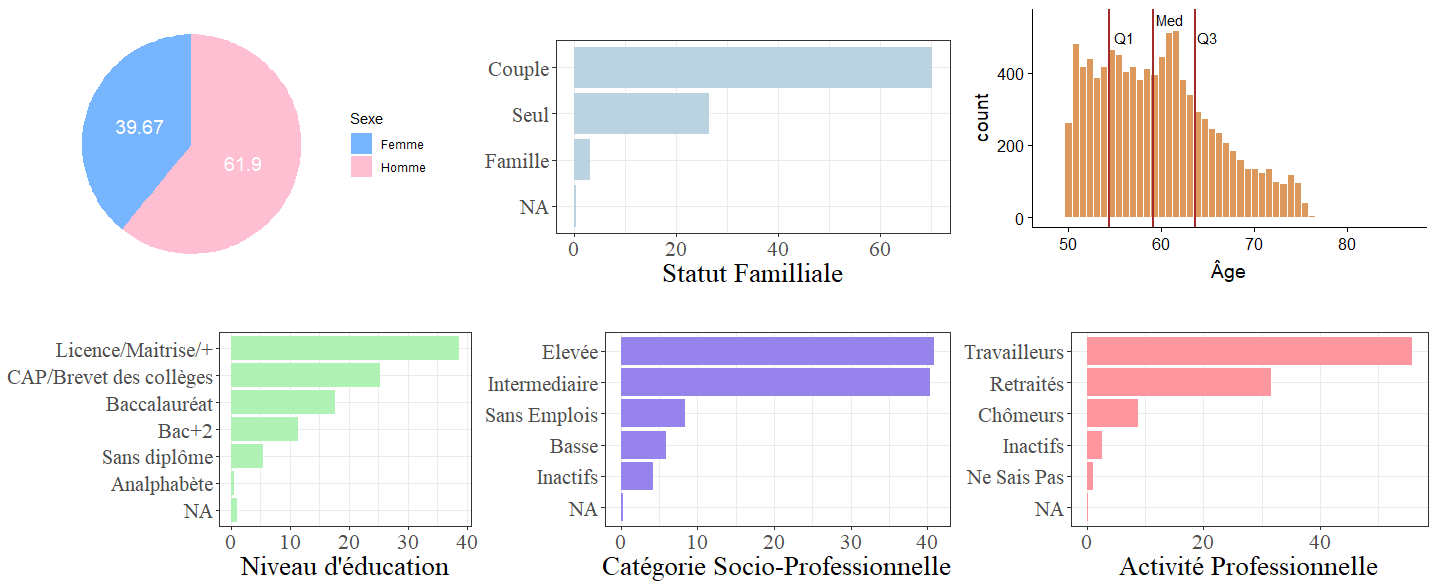
\includegraphics[scale=.4]{tab_var_socio_ad.png}
\end{center}
On observe ainsi que la cohorte EPP3 est masculine à plus de 60 $\%$. De plus pres de 70 $\%$ des individus déclarent vivre en couple tandis que 30 $\%$  déclarent vivre seuls et moins de 10 $\%$ en famille.\\

\noindent
Sans surprise l'histogramme des ages nous indique que les sujets sont globalement âgés de 50 à 75 ans (c'était un des critères d'inclusion). 50 $\%$ de la population a moins de 59 ans et 75 $\%$ moins de 63. Il n'est donc pas étonnant d'observer un peu plus de 25 $\%$ de Retraités contre un peu moins de 60 $\%$ de Travailleurs Actifs.\\

\noindent
Il est à noté que la distribution de l'âge ne semble pas suivre une lois normale. Cette hypothèse est confirmée après un test de Shapiro effectué sur des échantillons aléatoires d'individus de 5000 sujets.\\

Enfin la cohorte EPP3 se situe majoritairement dans les catégories socio-professionnelles élevée et intermédiaires.
Ils semblent de plus avoir un bon niveau d'éducation puisqu'à peine moins de 6 $\%$ se déclarent sans diplômes.\\

\bigskip
\item Variables Style de vie
\begin{center}
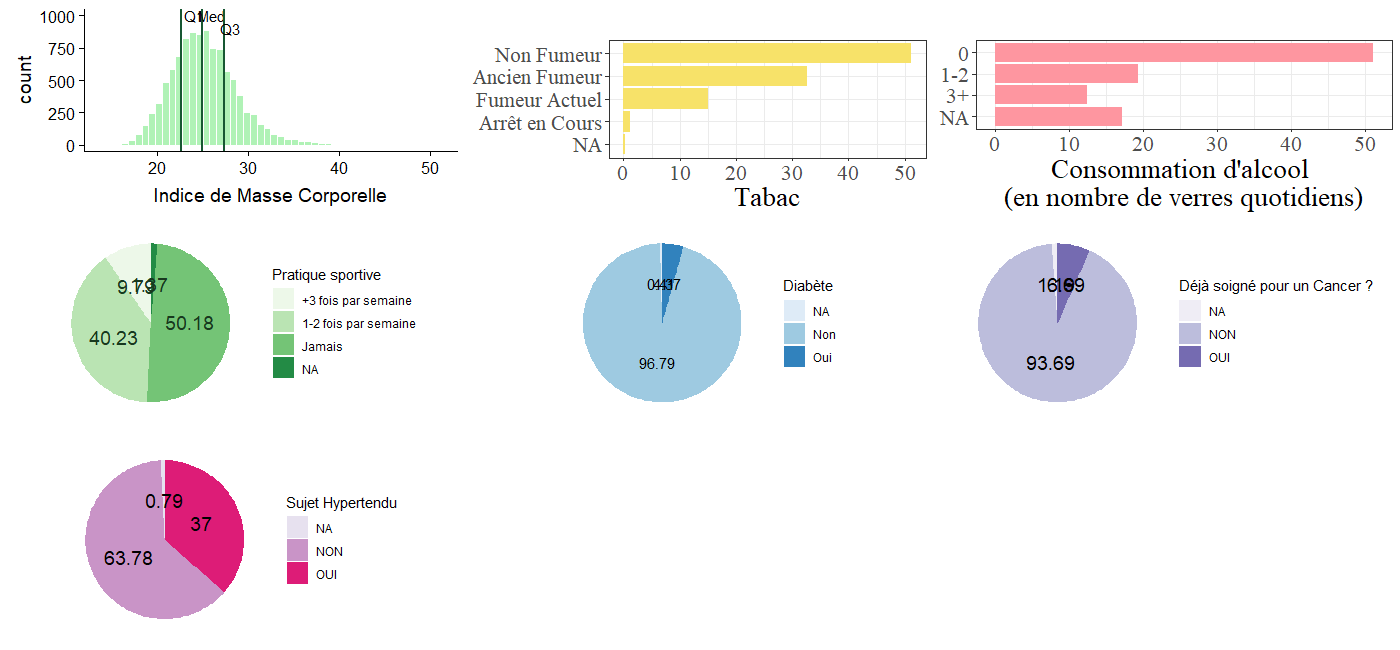
\includegraphics[scale=.45]{tab_var_sante_phys.png}
\end{center}

\noindent
La cohorte EPP3 est dans l'ensemble en bonne santé puisque globalement non diabètique $(> 96 ~ \%)$ et non cancéreuse $(> 96 \%)$.\\

\noindent
De plus une large majorité des sujets ne fume pas ou plus tandis que 70 $\%$ déclarent boire au plus 2 verres d'alcool par jours (tout alcool confondus).\\

\noindent
Cependant une part non négligeable des sujets est hypertendue mais très peu d'individus déclarent être atteint d'une maladie cardiovasculaire.\\

\bigskip
\item Variables Santé Psychique
\begin{center}
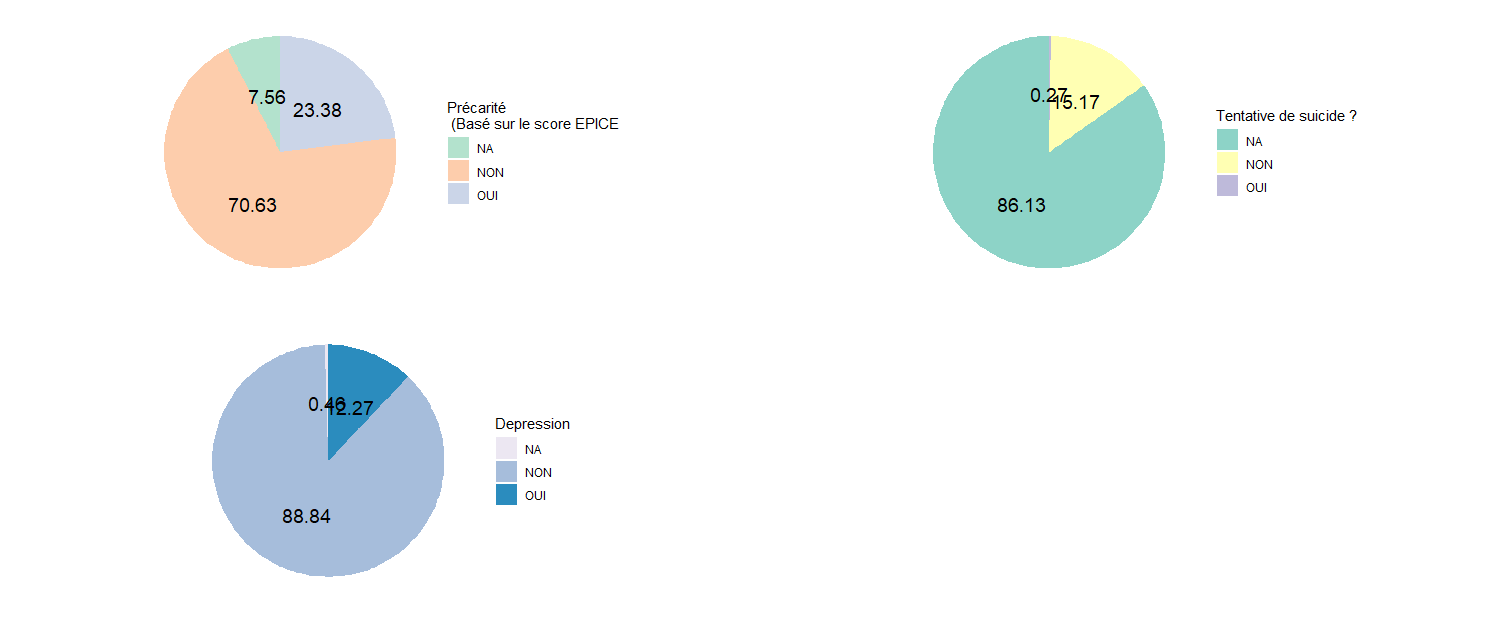
\includegraphics[scale=.4]{tab_var_sante_psy.png}
\end{center}
Enfin, on observe que très peu d'individus sont dépressifs mais que plus de 20 $\%$ sont en situation de précarité.
\end{enumerate}



%\begin{center}
%\setlength\arrayrulewidth{.6pt}
%\arrayrulecolor{black}
%\begin{tabular}{|c|c|c|c|c|c|c|c|}
%\hline
 %& Min & Mean & Max & Q1 & Median & Q3 & NA \\
 %\hline
 %\hline
 %Âge &  48.53 & 59.62 & 86.24 & 54.47 & 59.11 & 63.66 & 0\\
 %\hline
 %Indice de Masse Corporelle & 14.50 & 25.19 & 51.06 & 22.66 &  24.91 & 27.34 & 0\\
 %\hline
 %Score EPICE de précarité & 0 & 18.31 & 100 & 0 & 13.61 & 30.17 & 756\\
 %\hline
%\end{tabular}
%\end{center}

 
%Parler de la dif ci dessous, afficher table de contingence, conclure sur le biais évident des mesures subjectives !!!! 
%La variable dépression prend en compte à la fois le score de dépression (si sup à 7) et les antidépresseurs que les sujets déclarent prendre. 
%D'autre part il est demandé aux sujets s'ils ont déjà été diagnostiqué  par un médecin. Lorsque l'on compare les 2 variables on constate un écart de 1267 sujets.
 
 
\subsection{Données Manquantes}

\begin{center}
\noindent
Ci dessous, le tableau du nombre de données manquantes pour chacune des variables de l'analyse.\\
\bigskip

\begin{tabular}{rrl}
\toprule
Nb Na & \% NA & Variables\\
\midrule

1744 & 17.17 & Alcool (Nb de verres)\\
756 & 7.44 & Score Epice de Précarité\\
137 & 1.35 & Sport\\

134 & 1.32 & Maladies Cardiovasculaires\\
119 & 1.17 & Cancer\\
108 & 1.06 & Niveau d'Education\\
86 & 0.85 & Score de Stresse Perçu (PSS4)\\
79 & 0.78 & Hypertension Arterielle\\

46 & 0.45 & Depression\\
42 & 0.41 & Situation Familliale\\
41 & 0.40 & Diabète\\
30 & 0.30 & Catégorie Socio-Professionnelle\\

29 & 0.29 & Activité Professionnelle (CAH)\\
26 & 0.26 & Santé Perçue Binaire\\
20 & 0.20 & Tabac\\
16 & 0.16 & Activité Professionnelle (Codage Manuel)\\
1 & 0.01 & Âge\\

0 & 0.00 & Sexe\\
0 & 0.00 & Indice de Masse Corporelle(Classes)\\
\bottomrule
\end{tabular}
\end{center}

\noindent
Le nombre de données manquantes par variable de dépasse jamais les 20 $\%$, j'ai donc décider d'exclure les individus ayant au moins une des variables ci-dessus non renseignée.\\

\newpage
\section{Statistiques}
\subsection{Flowchart}

\begin{center}
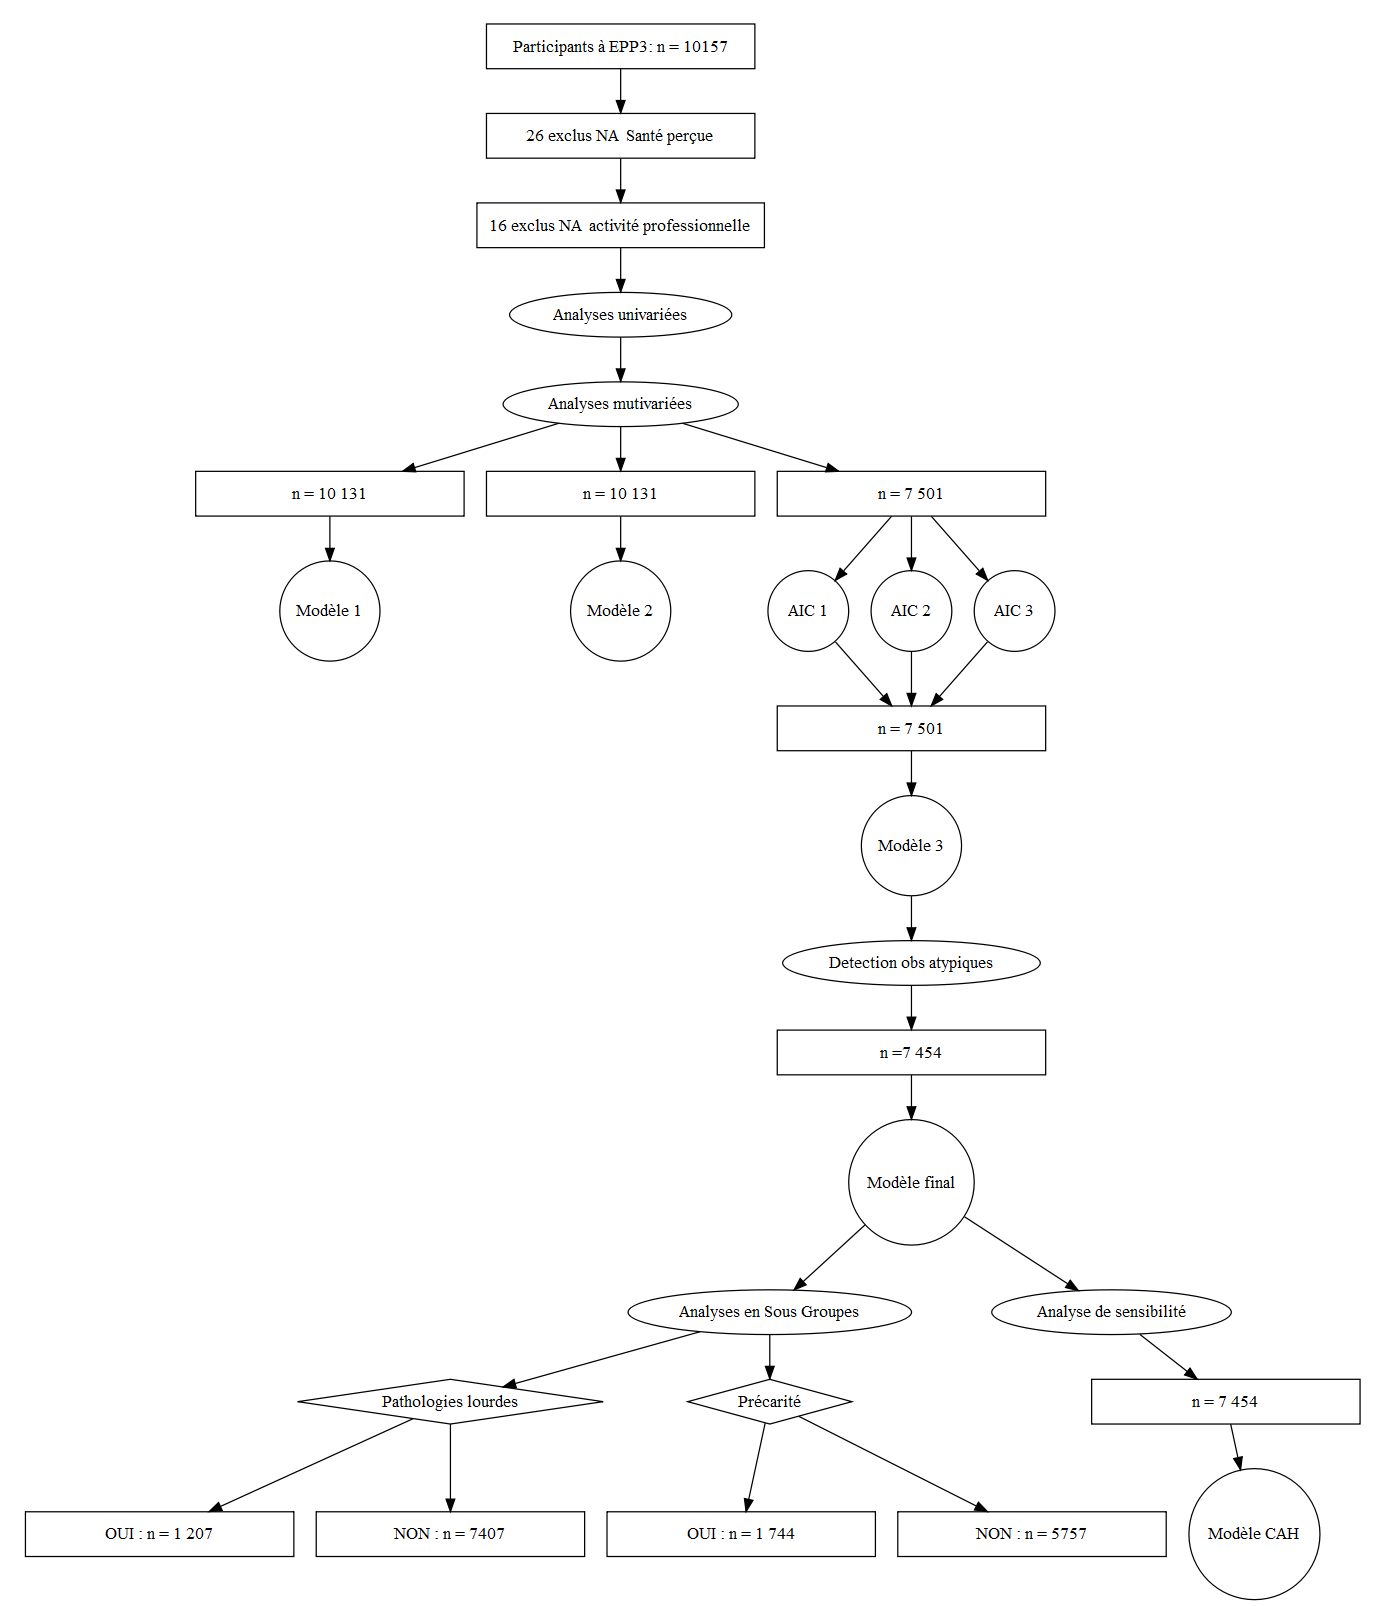
\includegraphics[scale=.25]{flowchart.png}
\end{center}


\subsection{Analyses univariées}

\noindent
Afin d'avoir une première idée des variables significativement liées à la santé perçue on effectue une régression logistique entre la santé perçue binarisée des sujets (on coupe à la médiane: si la santé perçue est > à 7 on la considère comme bonne) et chacune des variables explicatives.\\


\newpage

\noindent
\textbf{La régression logistique:}
\bigskip

\noindent
On cherche à modéliser la probabilité qu'une variable prenne une certaine valeur en fonction de variables explicatives.\\
La spécificité de la régression logistique est le caractère dichotomique de la variables à expliquer. Cela permet de modéliser l'appartenance à une classe de la variable à expliquer par une loi de Bernouilli.\\

\bigskip 

\noindent
Soit $Y$ la variables à expliquer et  $X_1, X_2,...X_p$ les $p$ variables explicatives.\\
On note $Y_i$ l'observation de la variable $Y$ pour l'individu $i$, $i \in  \ldbrack 0,n \rdbrack $(où $n$ est le nombre total d'individus) et $X_i = {(X_{i1}, X_{i2}, ..., X_{ip})}^t$ le vecteur des variables explicatives pour le sujet.\\
On note $\beta = {(\beta_0, \beta_1, \beta_2, ..., \beta_p)}^t$, le vecteur de dimension $p+1$ des paramètres du modèle.

\bigskip

\noindent
Le modèle logistique ne fait qu'une seule hypothèse à priori: \\
\begin{align*}
Y_i ~ iid \sim \mathfrak{B} (\pi(X_i))
\end{align*}
Où :
\begin{align*}
\pi(X_i) =& ~ \mathbb{E}(Y_i|X_i) \\
=& ~ \mathbb{P}(Y_i = 1|X_i) \\
=& ~ {e^{(\beta_0 + \sum_{k=1}^p {\beta_k X_{ik}})}} \over {1+{e^{(\beta_0 + \sum_{k=1}^p {\beta_k X_{ik}})}}}\\
=& ~ sigmoïde({e^{(\beta_0 + \sum_{k=1}^p {\beta_k X_{ik}})}})
\end{align*}
Ainsi on peut écrire:
\begin{align*}
Logit(\pi(X_i)) = & \log(\pi(X_i)) \over {1- \pi(X_i)} \\
=& \beta_0 + \sum_{k=1}^p {\beta_k X_{ik}}
\end{align*}

\noindent
$\forall k \in \ldbrack 1,p \rdbrack, e^{\beta_k}$ est l'odd ratio de la variable $k$.\\
\bigskip

\noindent
L'estimation du vecteur de régression se fait par la méthode du maximum de vraisemblance:
\begin{align*}
\mathfrak{L}(\beta) =& ~ \prod_{i=1}^n \left[
{\left(  {{e^{(\beta_0 + \sum_{k=1}^p {\beta_k X_{ik}})}} \over {1+{e^{(\beta_0 + \sum_{k=1}^p {\beta_k X_{ik}})}}}  } \right)}^{Y_i} {\left( 1 \over {1+ {e^{(\beta_0 + \sum_{k=1}^p {\beta_k X_{ik}})}}}   \right)}^{(1-Y_i)} \right]
\end{align*}
Ainsi: 
\begin{align*}
\log \left( \mathfrak{L}(\beta) \right)  = 
\sum_{k=1}^n {\left[ Y_i \left( \beta_0 + \sum_{k=1}^p {\beta_k X_{ik}}  \right) 
- \log \left( 1 + e^{\beta_0 +  \sum_{k=1}^p {\beta_k X_{ik}}  } \right)
\right]} \\
\end{align*}
Et donc $ \forall k \in \ldbrack 0,p \rdbrack :  $
\begin{align*}
{{\partial  \log \left( \mathfrak{L}(\beta) \right)} \over {\partial \beta_k} }= 
\sum_{i=1}^n {X_{ik} \left( Y_i - {{e^{X_i^t \beta}} \over {1+ e^{X_i^t \beta}}} \right)}
\end{align*}
Avec $X_{i0} = 1 $ et $ X_i^t \beta = \sum_{k = 1}^p {\beta_k X_{ik}} $

\bigskip

\noindent
L'équation $ {{\partial  \log \left( \mathfrak{L}(\beta) \right)} \over {\partial \beta} } = 0  $, qui permet d'obtenir $\hat{\beta}$, est résolue grâce à des algorithmes itératifs.\\

\bigskip

\noindent
On a de plus $\forall k \in \ldbrack 0,p \rdbrack$ :
\begin{align*}
\hat{\beta_k} \underset{n \rightarrow \infty}{\sim} \mathcal{N} \left( \beta_k,\widehat{\mathbb{V}} \left(  \hat{\beta_j}\right) \right)
\end{align*}

\bigskip

\noindent
Ainsi au niveau de confiance $-\alpha$ on a :
\begin{align*}
IC \left( \beta_k \right) =
 \left[
  \hat{\beta_k} \pm |z_{{\alpha} \over {2}}| \sqrt{\widehat{\mathbb{V}}\left( \hat{\beta_k} \right)}
\right]\\
\end{align*}

\noindent
Où $ z_{ {\alpha} \over {2}} $ est t.q $ \mathbb{P}\left( Z <  z_{ {\alpha} \over {2}} \right) = {{\alpha} \over {2}}$ pour $ Z \sim \mathcal{N}(0,1) $

\bigskip

\noindent
On a alors les intervalles de confiance des odd ration pour chacune des variables:\\
\begin{align*}
IC \left( e^{\beta_k} \right)  =& ~ IC \left( OR_k \right) \\
= & ~ e^{\left[ \hat{\beta_k} \pm |z_{{\alpha} \over {2}}| \sqrt{\widehat{\mathbb{V}}\left( \hat{\beta_k} \right)} \right]} \\
= & ~
 \left[
e^{\hat{\beta_k} - |z_{{\alpha} \over {2}}| \sqrt{\widehat{\mathbb{V}}\left( \hat{\beta_k} \right)}} 
~;~ 
e^{\hat{\beta_k} + |z_{{\alpha} \over {2}}| \sqrt{\widehat{\mathbb{V}}\left( \hat{\beta_k} \right)}} 
\right]
\end{align*}

\bigskip
\noindent
Ici la variable $Y$ est la santé perçue binarisée, les autres variables sont $p = 16 $ variables explicatives.

\bigskip

\noindent
J'ai choisi de catégoriser 3 des variables continues (IMC, âge et score épice de précarité afin de rendre l'interprétation des résultats plus évidente).\\
Ainsi l'âge a été découpé en quartiles.\\
Pour l'indice de masse corporelle, après discussion avec des médecins j'ai fixé à 25 le seuil de normalité et à 30 le seuil de sur poids. Au delà de 30 on parle d'obésité.\\
Enfin, le score de précarité a un seul officiel, comme expliqué plus haut les sujets ayant un score supérieur à 30.17 sont considéré en situation de précarité.\\


\newpage

    \begin{longtable}{lcccc}\caption{Analyses univariées}\\
    \hline  
     &      0       &      1       & \multirow{2}{*}{       OR       } & \multirow{2}{*}{p.ratio}\\ 
 &    N=4390    &    N=5741    &                  &         \\ 
  
    \hline
    \hline     
    \endfirsthead 
    \multicolumn{5}{l}{\tablename\ \thetable{} \textit{-- continued from previous page}}\\ 
    \hline
     &      0       &      1       & \multirow{2}{*}{       OR       } & \multirow{2}{*}{p.ratio}\\ 
 &    N=4390    &    N=5741    &                  &         \\ 

    \hline
    \hline  
    \endhead   
    \hline
    \multicolumn{5}{l}{\textit{continued on next page}} \\ 
    \endfoot   
    \multicolumn{5}{l}{}  \\ 
    \endlastfoot  
Activité Professionnelle: &              &              &                  &        \\ 
$\qquad$Travailleurs & 2446 (55.7\%) & 3213 (56.0\%) &       Ref.       &  Ref.  \\ 
$\qquad$Retraités & 1315 (30.0\%) & 1892 (33.0\%) & 1.10 [1.00;1.20] &  0.042 \\ 
$\qquad$Chômeurs & 424 (9.66\%)  & 458 (7.98\%)  & 0.82 [0.71;0.95] &  0.007 \\ 
$\qquad$Inactifs & 142 (3.23\%)  & 128 (2.23\%)  & 0.69 [0.54;0.88] &  0.003 \\ 
$\qquad$Ne Sais Pas &  63 (1.44\%)  &  50 (0.87\%)  & 0.60 [0.41;0.88] &  0.008 \\ 
Activité Professionnelle (CAH): &              &              &                  &        \\ 
$\qquad$Travailleurs & 2364 (53.9\%) & 3089 (53.9\%) &       Ref.       &  Ref.  \\ 
$\qquad$Chômeurs & 403 (9.19\%)  & 438 (7.64\%)  & 0.83 [0.72;0.96] &  0.013 \\ 
$\qquad$Inactifs & 210 (4.79\%)  & 206 (3.59\%)  & 0.75 [0.61;0.92] &  0.005 \\ 
$\qquad$Retraités & 1408 (32.1\%) & 2000 (34.9\%) & 1.09 [1.00;1.19] &  0.059 \\ 
Sexe: &              &              &                  &        \\ 
$\qquad$Hommes & 2424 (55.2\%) & 3750 (65.3\%) &       Ref.       &  Ref.  \\ 
$\qquad$Femmes & 1966 (44.8\%) & 1991 (34.7\%) & 0.65 [0.60;0.71] &  0.000 \\ 
Situation Familiale: &              &              &                  &        \\ 
$\qquad$Couple & 2929 (66.8\%) & 4180 (73.1\%) &       Ref.       &  Ref.  \\ 
$\qquad$Famille & 134 (3.06\%)  & 188 (3.29\%)  & 0.98 [0.78;1.23] &  0.881 \\ 
$\qquad$Seul & 1320 (30.1\%) & 1354 (23.7\%) & 0.72 [0.66;0.79] & $<$0.001 \\ 
Âge: &              &              &                  &        \\ 
$\qquad$ $\leq$ 54 & 1134 (25.8\%) & 1395 (24.3\%) &       Ref.       &  Ref.  \\ 
$\qquad$ ]54,59] & 1140 (26.0\%) & 1393 (24.3\%) & 0.99 [0.89;1.11] &  0.906 \\ 
$\qquad$ ]59,63] & 1051 (23.9\%) & 1482 (25.8\%) & 1.15 [1.03;1.28] &  0.016 \\ 
$\qquad$ $\>$ & 1065 (24.3\%) & 1470 (25.6\%) & 1.12 [1.00;1.25] &  0.042 \\ 
Éducation: &              &              &                  &        \\ 
$\qquad$CAP/Brevet des collèges & 1212 (27.9\%) & 1354 (23.8\%) &       Ref.       &  Ref.  \\ 
$\qquad$Analphabète &  26 (0.60\%)  &  24 (0.42\%)  & 0.83 [0.47;1.45] &  0.508 \\ 
$\qquad$Bac+2 & 485 (11.2\%)  & 662 (11.6\%)  & 1.22 [1.06;1.41] &  0.005 \\ 
$\qquad$Baccalauréat & 812 (18.7\%)  & 977 (17.2\%)  & 1.08 [0.95;1.22] &  0.230 \\ 
$\qquad$Licence/Maitrise/+ & 1500 (34.5\%) & 2435 (42.8\%) & 1.45 [1.31;1.61] & $<$0.001 \\ 
$\qquad$Sans diplôme & 313 (7.20\%)  & 239 (4.20\%)  & 0.68 [0.57;0.82] & $<$0.001 \\ 
Catégorie Socio-Professionnelle: &              &              &                  &        \\ 
$\qquad$Intermédiaire & 1908 (43.5\%) & 2186 (38.1\%) &       Ref.       &  Ref.  \\ 
$\qquad$Basse & 300 (6.84\%)  & 294 (5.13\%)  & 0.86 [0.72;1.02] &  0.076 \\ 
$\qquad$Élevée & 1541 (35.2\%) & 2605 (45.4\%) & 1.48 [1.35;1.61] &  0.000 \\ 
$\qquad$Inactifs & 219 (5.00\%)  & 207 (3.61\%)  & 0.83 [0.68;1.01] &  0.059 \\ 
$\qquad$Sans Emplois & 416 (9.49\%)  & 441 (7.69\%)  & 0.93 [0.80;1.07] &  0.302 \\ 
Indice de Masse Corporelle: &              &              &                  &        \\ 
$\qquad$Normal & 2080 (47.4\%) & 3105 (54.1\%) &       Ref.       &  Ref.  \\ 
$\qquad$Obésité & 551 (12.6\%)  & 427 (7.44\%)  & 0.52 [0.45;0.60] &  0.000 \\ 
$\qquad$Sur-poids & 1759 (40.1\%) & 2209 (38.5\%) & 0.84 [0.77;0.91] & $<$0.001 \\ 
Tabac: &              &              &                  &        \\ 
$\qquad$Non Fumeurs & 2269 (51.7\%) & 2919 (50.9\%) &       Ref.       &  Ref.  \\ 
$\qquad$ Ancien Fumeurs & 1327 (30.2\%) & 1979 (34.5\%) & 1.16 [1.06;1.27] &  0.001 \\ 
$\qquad$Arrête en Cours &  61 (1.39\%)  &  49 (0.85\%)  & 0.62 [0.43;0.91] &  0.015 \\ 
$\qquad$ Fumeurs & 733 (16.7\%)  & 790 (13.8\%)  & 0.84 [0.75;0.94] &  0.002 \\ 
Diabète: &              &              &                  &        \\ 
$\qquad$Non & 4132 (94.3\%) & 5537 (96.7\%) &       Ref.       &  Ref.  \\ 
$\qquad$Oui & 250 (5.71\%)  & 187 (3.27\%)  & 0.56 [0.46;0.68] & $<$0.001 \\ 
Activité Sportive: &              &              &                  &        \\ 
$\qquad$Jamais & 2531 (58.4\%) & 2480 (43.7\%) &       Ref.       &  Ref.  \\ 
$\qquad$1-2 fois par semaine & 1524 (35.2\%) & 2496 (44.0\%) & 1.67 [1.54;1.82] &  0.000 \\ 
$\qquad$ $\geq$ 3 fois par semaine & 277 (6.39\%)  & 702 (12.4\%)  & 2.59 [2.23;3.01] &  0.000 \\ 
Hypertension Artérielle: &              &              &                  &        \\ 
$\qquad$Non & 2564 (58.9\%) & 3801 (66.7\%) &       Ref.       &  Ref.  \\ 
$\qquad$Oui & 1792 (41.1\%) & 1898 (33.3\%) & 0.71 [0.66;0.78] & $<$0.001 \\ 
Consommation d'alcool: &              &              &                  &        \\ 
$\qquad$0 & 2262 (63.7\%) & 2922 (60.1\%) &       Ref.       &  Ref.  \\ 
$\qquad$1-2 & 759 (21.4\%)  & 1205 (24.8\%) & 1.23 [1.11;1.37] & $<$0.001 \\ 
$\qquad$3+ & 528 (14.9\%)  & 734 (15.1\%)  & 1.08 [0.95;1.22] &  0.248 \\ 
Cancer: &              &              &                  &        \\ 
$\qquad$Non & 3997 (91.9\%) & 5364 (94.5\%) &       Ref.       &  Ref.  \\ 
$\qquad$Oui & 354 (8.14\%)  & 315 (5.55\%)  & 0.66 [0.57;0.78] & $<$0.001 \\ 
Score EPICE de précarité: &              &              &                  &        \\ 
$\qquad$Situation non précaire & 2827 (69.5\%) & 4230 (79.5\%) &       Ref.       &  Ref.  \\ 
$\qquad$Situation précaire & 1240 (30.5\%) & 1094 (20.5\%) & 0.59 [0.54;0.65] &  0.000 \\ 
Dépression: &              &              &                  &        \\ 
$\qquad$Non & 3533 (80.7\%) & 5344 (93.4\%) &       Ref.       &  Ref.  \\ 
$\qquad$Oui & 847 (19.3\%)  & 377 (6.59\%)  & 0.29 [0.26;0.33] &  0.000 \\ 
Score de stresse perçu (PSS4)

 $\qquad$ & .  & .  &0.82 [0.81;  0.84] &  < 2.2e-16 \\ 
    \hline
    \end{longtable} 

\bigskip

\noindent
On remarque un lien significatif entre l'activité professionnelle et la santé perçue et ce, que l'on considère la classification manuelle ou la classification ascendante hiérarchique de la variable activité professionnelle. Ainsi, les retraités ont une santé perçue de 10 $\%$ supérieure aux travailleurs tandis que la SRH des chômeurs est 40 $\%$ moins bonne et celle des inactifs 30 \$%$ moins bonne. \\

\noindent
Le groupe des individus non classés manuellement (NSP) s'apparente aux inactifs en terme de baisse de santé perçue. Ce résultat est cohérent avec l'observation faite plus haut : la CAH classe majoritairement ces individus en inactifs.\\
\bigskip
\noindent
Les femmes ont une santé perçue de 35 $\%$ inférieure à celle des hommes. On peut peu-être expliquer cela par le fait que les grossesses rendent la santé des femmes plus fragile. De plus certaines études montrent que les femmes sont plus enclines à la dépression que les hommes \cite{nolen2001gender}. Or la santé perçue des sujets dépressifs est de 70 $\%$ inférieure à celle des sujets non dépressifs.\\
\bigskip

\noindent
Un résultat intéressant est le lien entre la santé perçue et l'entourage du sujet. Les individus déclarant vivre seuls ont une santé perçue significativement inférieure à celle des sujets en couple.\\ Il aurait été éclairant de pouvoir tester cette liaison plus en profondeur, par exemple en demandant aux individus de noter leur sentiment de bonheur au quotidien et d'ensuite coupler ces résultats avec le fait de vivre en couple ou non.\\
\bigskip

\noindent
Sans surprise on observe que les sujets ayant une catégorie scio-professionnelle basse se perçoivent en moins bonne santé que ceux de la classe intermédiaire (de même que les inactifs comme nous l'avons déjà vu grâce à la variable d'activité professionnelle), tandis que les sujets d'une CSP élevée voient leur santé perçue augmentée de 50 $\%$. On peut facilement imaginer que plus on descend dans les catégories socio-professionnelles, plus l'accès au soin dans son sens le plus large (ne serait-ce que l'accès à l'information de santé et à la prévention) est difficile.\\
\bigskip

\noindent
Dans le même ordre d'idée les sujets de la cohorte se perçoivent en meilleur santé lorsqu'ils ont eu un parcours éducatif plus long. Ainsi les détenteurs d'un BAC+2 ont une santé perçue de 22 $\%$ supérieure à ceux ayant un CAP ou le brevet des collèges. Cette augmentation passe à 45 $\%$ pour les détenteurs d'une licence ou d'un autre diplôme supérieur. Toutefois les sujets ne sachant ni lire ni écrire voient leur santé perçue baisser de plus de 20 $\%$ par rapport aux diplômés d'un CAP ou d'un Brevet des collèges.\\
\bigskip


\noindent
Parmi les variables décrivant la santé réelle des sujets de l'étude, observons que les fumeurs ont une santé perçue de plus de 15 $\%$ inférieure à celle des non fumeurs. Il est intéressant de remarquer que les anciens fumeurs s'estiment en meilleur santé que ceux qui sont non fumeurs (augmentation de 20 $\%$). Cela s'explique peut-être par le fait que ces individus ont vu un réel effet de l'arrêt du tabac sur leur corps et qu'ils s'estiment, par conséquent, en très bonne santé à présent qu'ils ne fument plus.\\
Ce qui parait étonnant par contre c'est que les sujets déclarant être en période de sevrage ont une baisse de santé perçue plus importante que les les fumeurs par rapport aux sujets non fumeurs. La difficulté psychologique de l'arrêt de la cigarette ainsi que la prise de poids qui le suit souvent sont des explications probables.\\
\bigskip

\noindent
L'un des résultats les plus étonnants de cette analyse est celui concernant la consommation quotidienne d'alcool (en nombre de verres).\\
Par rapport aux abstinents, on trouve chez les sujets buvant entre 1 et 2 verres d'alcool par jour une augmentation significative de plus de 20 $\%$ de la santé perçue. On pourrait expliquer ce phénomène par le plaisir de boire un verre entre amis ou avec son conjoint. S'il est impossible de vérifier que les individus déclarant boire 1 à 2 verres par jour boivent seuls ou avec des amis ou de la famille, on peut cependant remarquer que la grande majorité de ces individus vivent en couple et qu'ils sont pour la plupart non dépressifs (ils ont donc probablement moins tendance à s'isoler et ont donc plus probablement une vie sociale développée).

\begin{center}
\setlength\arrayrulewidth{.1pt}
\arrayrulecolor{black}
\begin{tabular}{cc}
\setlength\arrayrulewidth{.1pt}
\begin{tabular}{|l|r|}
\hline
couple & 1472\\
\hline
famille & 61\\
\hline
seul & 426\\
\hline
\end{tabular}
&
\begin{tabular}{|l|r|}
\hline
0 & 1767\\
\hline
1 & 196\\
\hline
NA & 3\\
\hline
\end{tabular}
\end{tabular}
\end{center}

\subsection{Analyses multivariées}
\subsubsection{Régression logistique}

\noindent
On prend en compte dans le modèle l'ensemble des variables décrites dans l'analyse univariée puisque cette dernière montre qu'elles sont toutes significatives.\\

\noindent
Nous avions précédemment établi que l'âge était un facteur de confusion évident pour le lien entre la santé perçue et l'activité professionnelle: la comparaison des deux modèles suivants le montre assez clairement:

\begin{longtable}{lccc|ccc}\caption{Mise en évidence de l'âge comme facteur de confusion}\\
    \hline  
    		 & &    Modèle 1 &   &    &   Modèle 2    &\\
		& \multirow{3}{*}{OR} & \multirow{3}{*}{IC}& \multirow{3}{*}{p} & \multirow{3}{*}{OR} & \multirow{3}{*}{IC}& \multirow{3}{*}{p}\\ 
		 &      &     &    &   	    &  	    &\\
   \hline
    \hline     
    \endfirsthead 
    \multicolumn{4}{l}{\tablename\ \thetable{} \textit{-- continued from previous page}}\\ 
    \hline
	    		 & &    Modèle 1 &   &   &   Modèle 2    &\\
		& \multirow{3}{*}{OR} & \multirow{3}{*}{IC}& \multirow{3}{*}{p} & \multirow{3}{*}{OR} & \multirow{3}{*}{IC}& \multirow{3}{*}{p}\\ 
		 &      &     &    &   	    &  	    &\\
    \hline
    \hline  
    \endhead   
    \hline
    \multicolumn{4}{l}{\textit{continued on next page}} \\ 
    &    				    &    			    &                  \\ 
    \endfoot   
    \multicolumn{4}{l}{}  \\ 
    \endlastfoot 
        
Intercept & 1.52 & $\left[1.43 ; 1.62 \right]$ & <2.2e-16 & 1.44 & $\left[1.33 ; 1.57 \right]$ & <2.2e-16\\
Activité Professionnelle: &              &              &	&&&\\ 
$\qquad$Travailleurs 		&		Ref.		& 	Ref.		&	Ref.&Ref.&Ref.&Ref.\\ 
$\qquad$Retraités&1.15 &$\left[1.05 ; 1.26 \right]$ & 0.002&1.06 &$\left[0.94 ; 1.20 \right]$ & 0.36\\ 
$\qquad$Chômeurs & 0.82& $\left[0.71 ; 0.95\right]$& 0.006 & 0.81& $\left[0.70 ; 0.94\right]$& 0.004\\ 
$\qquad$Inactifs  & 0.88& $\left[0.68 ; 1.13\right]$& 0.30 & 0.84& $\left[0.65 ; 1.08\right]$& 0.18\\  
$\qquad$Ne Sais Pas & 0.68& $\left[0.47 ; 0.99\right]$ & 0.048& 0.66& $\left[0.45 ; 0.97\right]$ & 0.03 \\
Sexe: &              &              &                        &&&  \\ 
$\qquad$Hommes &Ref. & Ref.& Ref.&Ref.&Ref.&Ref.\\ 
$\qquad$Femmes & 0.65& $\left[0.6 ; 0.71 \right]$ & <2.2 e-16& 0.65& $\left[0.6 ; 0.71 \right]$ & <2.2 e-16\\
Âge: &&&&&&\\
$\qquad$<54.5 &&&&Ref.&Ref.&Ref.\\
$\qquad$ $\left[54.5 ; 59.1 \right]$&&& &1.04& $\left[0.93 ; 1.16 \right]$& 0.53\\
$\qquad$ $\left[59.1 ; 63.7\right]$&&& &1.18&$\left[1.04 ; 1.34 \right]$& 0.008\\
$\qquad$ $\left[63.7 ; 86.2 \right]$&&&&1.13&$\left[0.97 ; 1.31 \right]$&0.11\\  
 
 
    \hline
    \end{longtable} 

\noindent
Lorsque l'on n'ajuste pas le modèle sur l'âge, on montre que les retraités ont une meilleurs santé perçue que les travailleurs: augmentation de 15 $\%$ avec une p-valeur de 0.002.\\
Dés lors que l'on ajuste sur l'âge cette information est masquée par l'augmentation de 18 $\%$ de la santé perçue des sujets dont l'âge est compris entre 59 et 64 ans: tranche d'âge de près d'un tiers des retraités (97 $\%$ ont plus de 59 ans).

\bigskip

\noindent
Les variables considérées par l'étude peuvent être divisées en 3 catégories: celles qui traitent du style de vie des sujets (indice de masse corporelle, statut tabagique, diabète, pratique sportive, hypertension, consommation d'alcool), les variables "socio-administratives" (sexe, statut familiale, âge, niveau d'éducation, catégorie socio-professionnel, activité professionnelle) et celles traitant de la santé psychique des sujets (dépression, stresse).

\bigskip

\noindent
J'ai fait une sélection de variables dans chacun des trois blocs en me basant sur le critère AIC \footnote{$AIC = -2 \log \left( \mathfrak{L} (\hat{\beta}) \right) + 2p $} (méthode stepwise) en incluant dans chaque modèle l'activité professionnelle qui est notre variable d'exposition, l'âge et le sexe. Chacun des trois modèles élimine l'âge et conserve toutes les autres variables.

\bigskip

\noindent
On inclut ces dernières dans le modèle final:

\newpage

    \begin{longtable}{lccc}\caption{Modèle final}\\
    \hline  
     &                \multirow{2}{*}{OR}    & \multirow{2}{*}{IC} & \multirow{2}{*}{p}\\ 
 &     &                        &         \\ 
  
    \hline
    \hline     
    \endfirsthead 
    \multicolumn{4}{l}{\tablename\ \thetable{} \textit{-- continued from previous page}}\\ 
    \hline
    &                     \multirow{2}{*}{OR}    & \multirow{2}{*}{IC} & \multirow{2}{*}{p}\\ 
 &     &                     &         \\ 

    \hline
    \hline  
    \endhead   
    \hline
    \multicolumn{4}{l}{\textit{continued on next page}} \\ 
    \endfoot   
    \multicolumn{4}{l}{}  \\ 
    \endlastfoot

Intercepte : &2.90 & [2.42;3.47] &< 2.2e-16 \\    
Activité professionnelle:  &         &              &                         \\ 
$\qquad$Travailleurs & Ref.& Ref. & Ref.             \\ 
$\qquad$Retraités &1.20&[1.08;1.35] &0.001\\
$\qquad$Chômeurs   & 1.03& [0.42;2.61]& 0.95\\ 
$\qquad$Inactifs &0.99& [0.56;1.75] &0.99\\
$\qquad$NSP  &0.73&[0.39;1.34] &0.309\\ 

Sexe&&&\\
$\qquad$Hommes & Ref.& Ref. & Ref.             \\
$\qquad$Femmes &0.82 &[0.73;0.91] &0.0004\\
 
Catégorie socio-professionnelle&&&\\
$\qquad$Intermédiaire&&&\\
$\qquad$Basse &0.85& [0.52;1.42] &0.54\\ 
$\qquad$Elevée &0.87& [0.68;1.11] &0.25\\ 
$\qquad$Inactifs   &0.83& [0.73;0.93] &0.002\\
$\qquad$Sans Emplois &0.89 &[0.35;2.23] &0.81\\

 
Éducation&&&\\
$\qquad$CAP/Brevet des collèges &Ref.&Ref.&Ref.\\
$\qquad$Analphabète &1.45& [0.55;3.81] & 0.44 \\   
$\qquad$Bac+2       &1.04 & [0.88;1.24] & 0.66   \\  
$\qquad$Baccalauréat   &0.99& [0.86;1.16] & 0.98   \\        
$\qquad$Licence/Maitrise/+   &1.11 & [0.97;1.27] & 0.12 \\   
$\qquad$Sans diplôme   &0.77 & [0.60;0.97] & 0.03\\

         
Situation Familiale&&&\\
$\qquad$Couple&Ref.&Ref.&Ref.\\
$\qquad$Famille&1.01& [0.76;1.35]& 0.95\\    
$\qquad$Seul&0.94 & [0.84;1.05]& 0.26   \\

Activité Sportive&&&\\
$\qquad$Jamais & Ref.&Ref.&Ref.\\
$\qquad$1-2 fois par semaine&1.47& [1.32;1.62]& 1.03e-13\\
$\qquad$ $\geq$3 fois par semaine &2.38 &[1.99;2.84] &< 2.2e-16\\
                  

Indice de Masse Corporelle&&&\\
$\qquad$Normal &Ref.&Ref.&Ref.\\
$\qquad$Sur-poids &0.80 &[0.72;0.89]& 3.07e-05\\ 
$\qquad$Obésité&0.59& [0.49;0.70]& 1.03e-09\\ 

Hypertension Artérielle&&&\\
$\qquad$Non& Ref.&Ref.&Ref.\\
$\qquad$Oui &0.77 &[0.69;0.85]& 2.217e-07\\ 

Statut Tabagique&&&\\
$\qquad$Non fumeurs &Ref.&Ref.&Ref.\\
$\qquad$Ancien Fumeur &1.09& [0.98;1.21]& 0.12\\    
$\qquad$Arrêt en cours &0.56 &[0.35;0.88]& 0.01\\ 
$\qquad$Fumeurs actuels &0.92& [0.80;1.06]& 0.24\\

Dépression&&&\\
$\qquad$Non&Ref.&Ref.&Ref.\\
$\qquad$Oui & 0.47 &[0.39;0.55]& < 2.2e-16\\
Stresse &0.86& [0.85;0.88]& < 2.2e-16\\ 
\hline
\end{longtable}

\subsubsection{Diagnostique du modèle}

\noindent
Tout d'abord, vérifions le linéarité du lien entre la santé perçue binarisée est le stresse (unique covariable quantitative).\\
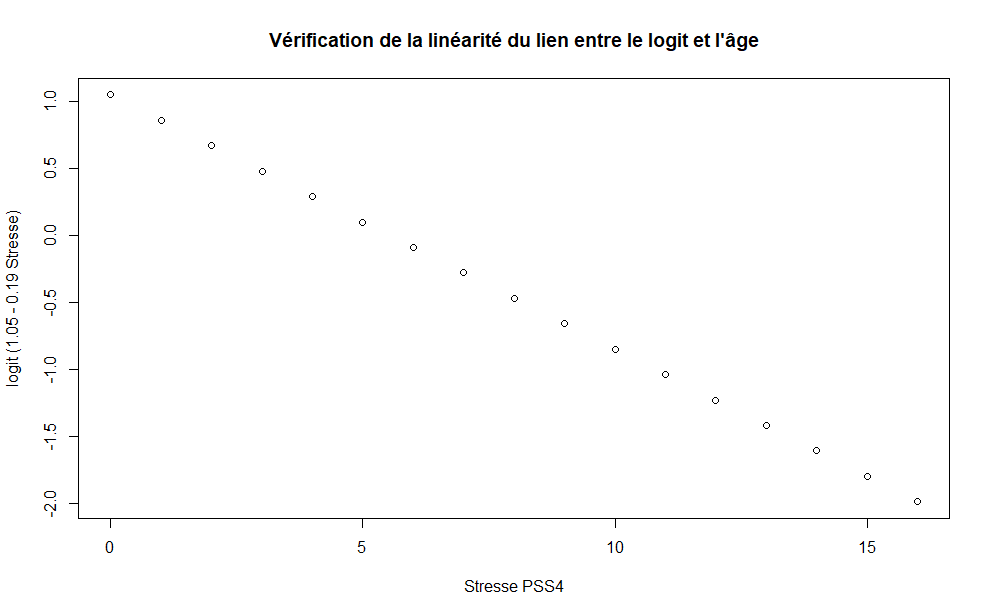
\includegraphics[scale=.7]{linearite_stresse.png}
Le Logit semble baisser lorsque le score de tresse augmente ce qui est logique puisque plus le PSS4 est élevé plus le sujet est considéré comme stressé.\\

\bigskip
\noindent
%Le modèle final établi précédemment est adéquat. en effet on a: $deviance(modèle final) \over %ddl.deviance(modèle final)} = 1.28$ qui est assez proche de 1.
\textbf{test des résidus de Pearson}\
$\forall i \in \ldbrack 1,n \lrbrack $ on a :
\begin{align*}
e_i = {  {Y_i - \widehat{\pi(X_i)}} \over {}  }
\end{align*}
$H_0$: Le modèle est adéquat.\\
$H_1$: Le modèle n'est pas adéquat.\

\subsection{Analyse en sous-groupes}
on applique le modele precedent en comprant a caque fois deux populations : celle qui possede un certain critere et celle qui ne le posse de pas.
\subsubsection{Pathologies lourdes}
\subsubsection{Score précarité}
\subsubsection{Âge}

\newpage
\section{Perspectives : Ce que j'ai fait, découvert, appris}

Comme expliqué plus haut, j'ai effectué mon stage dans l'unité INSERM 970 qui est spécialisée dans les maladies cardiovasculaires.\\
J'y ait passé cinq mois: du 01/04/2019 au 31/08/2019, durant lesquels j'ai beaucoup appris dans des domaines très variés.\\
Tout d'abord j'ai découvert le monde de la recherche, qui m'a beaucoup plu. C'était un monde entièrement neuf pour moi et la longue durée de mon stage a été un atout non négligeable dans son succès: en effet j'ai eu le temps de m'adapter à l'environnement, aux us et coutumes, au jargon, à l'équipe.\\

Cela m'a également donné le temps de me documenter sur l'épidémiologie: domaine qui m'était inconnu et qui, malgré sa ressemblance avec les statistique a ses propres règles, son propre vocabulaire.\\

En m'intégrant dans l'équipe, j'ai découvert le travail de groupe nécessaire à la rédaction de chaque article scientifique et l'émulsion que cela occasionne.
J'ai pu apprendre les grandes étapes de l'élaboration d'une étude épidémiologique, le cadre légal, le recrutement des individus, leur suivi ainsi que la saisie et le nettoyage des données.\\
J'ai également participé au recueil de certaines données en appelant les hôpitaux pour récupérer des comptes redus hospitaliers de sujets de l'étude qui étaient utiles aux médecins investigateurs pour confirmer une pathologie déclarée par lesdits sujets dans les questionnaires de suivis. J'ai ainsi pu me confronter à l'épineux problème de la confidentialité des données de santé.\\
J'ai également eu l'occasion de participer au reviewing d'un article (pas officiellement juste pour la pédagogie). J'ai ainsi pu apprendre toutes les étapes de la rédaction d'un article: le travail de recherche, la mise en forme des idée puis la recherche d'une revue susceptible de publier l'article, l'étape de relecture par des pairs et la prise en compte de leurs remarques...\\

Au delà du monde de la recherche, j'ai dû apprendre à m'intégrer dans un groupe où il y avait une grande pluralité des parcours (médecins, statisticiens, attachés de recherches cliniques, ingénieurs...). Cela supposait de se rendre intelligible par tous, et parfois de verser dans une forme de vulgarisation de certains concepts statistiques ce qui m'a beaucoup enrichie\footnote{Voir les chaînes Youtube StatQuest et science4all (notamment la série de vidéo sur la formule de Bayes) qui ne se contentent pas d'expliquer vaguement quelques concepts très connu mais qui vont au fond des choses tout en les rendant accessibles au "grand publique"}.\\
J'ai également beaucoup profité du savoir des médecins qui m'entouraient notamment sur le fonctionnement de la santé en France ainsi que sur certaines notions médicales élémentaires. Ainsi j'ai pu percevoir la différence entre une "jolie" analyse statistique et une analyse qui avait un sens/intérêt clinique.\\ 

Au niveau des statistiques, plutôt que de me lancer dans de techniques "avancées", mon directeur de stage et moi avons décider de nous concentrer sur les bases comme la visualisation de données et la régression logistique. J'ai pris l'initiative de tenter des méthodes exploratoires comme l'ACM ou la CAH.\\
Régulièrement l'équipe se réunissait pour des réunions de méthodologie durant lesquelles j'ai pu me familiariser avec d'autres notions dont j'espère étudier le versant mathématiques en M2 (modèles de suivi, méta-analyse, données répétées et GEE...).\\
Ces réunions avaient pour support un article dont on faisant une lecture critique en tentant de comprendre d'une part les intérêts clinique de l'étude menée et d'autre part les méthodes statistiques mises en œuvre.\\

Profitant du temps que j'avais, je me suis familiarisée avec de nouveaux outils qui se sont révélés trés utils: github pour le versionnage de mon code et de ce rapport, pubmed pour lire ce qui s'était déjà fait sur mon sujet et zotero pour créer ma bibliographie.

Pour conclure, ce stage était une très bonne expérience, très enrichissante qui m'a donné envie de poursuivre dans la recherche en en bio-satistiques.\\

\begin{center}
\section*{Conclusion}
Conclusion on verra à la fin:

Reste à faire: 

Il faut aussi mettre la méthode maths de l'ACM\\
Dans la partie sur la CAH: ajouter les equations maths de distance chi2 et critère de ward.\\
Appliquer consolidation par k means et adapter la rédaction qui suit (la ou on décrit le résultats sur le classf qui vont forcement changer puisqu'on ajoute une autre méthode de classif)\\
Décrire la méthode des k means. Préciser qu'on perd la hiérarchisation mais que cela permet de rendre la CAH plus stable. Expliquer que utiliser le k means en premier n'était pas une bonne idée car il fallait déterminer x0 et que je n'avais aucune idée de comment faire un choix pertinent. (en plus k means très sensible à l'initialisation: pas cool)\\

Il faut faire un compareGroups sur la ppo totale et pop-exclus.\\S
Il faut également, dans la partie statistique inclure un récap sur ce qu'est la régression logistique 
Dernières choses: mettre ne annexe le questionnaire ipc et la feuille d'évaluatoion de Jean Philippe.\\
Ne pas oublier de rediger la bibliographie.\\
\end{center}

\backmatter
\section{Annexes}
\section{Bibliographie}

\bibliographystyle{plain}
\bibliography{bib_stage}
\end{document}
